\documentclass[12pt,a4paper]{article}
\usepackage[utf8]{inputenc}
\usepackage{graphicx}
\usepackage{amsmath}
\usepackage{amsthm}
\usepackage{amssymb}
\usepackage{hyperref}
\usepackage{subfig}
\usepackage{multirow}

\begin{document}

\begin{titlepage}
	\centering
	
\includegraphics[width=0.15\textwidth]{IIIT-B_logo.jpg}\par\vspace{1cm}
	{\scshape\LARGE International Institute of Information Technology Bangalore \par}
	\vspace{1cm}
	{\scshape\Large Project Progress Report\par}
	{\Large DS/NC/ESD 863 Machine Perception\par}
	\vspace{1.5cm}
	{\huge\bfseries Vehicle Driving Assistant \par}
	\vspace{2cm}	   
	{\Large\itshape Akanksha Dwivedi - MT2016006\par}
	{\Large\itshape Anoop Toffy - MT2016016\par}
	{\Large\itshape Athul Suresh - MT2016030\par}
	{\Large\itshape Tarini Chandrashekhar - MT2016144\par}
	\vfill
	{\huge Group 7 \par}
	\vfill
	Guide : \par
	Prof. Dinesh Babu Jayagopi 

	\vfill

% Bottom of the page
	{\large \today\par}
\end{titlepage}


\tableofcontents
\listoffigures
%\listoftables
\newpage

\section{Problem Statement}
The project aims to provide a comprehensive set of assistance features to aid the driver (or autonomous vehicle) to drive safely. This includes a number of indicators about the environment, the major cue being detection of potholes in the road ahead.


\section{Motivation}
Autonomous vehicles has been a common term in our day to day life with car manufacturers like Tesla shipping cars that are SAE Level 3. While these vehicles include a slew of features such as parking assistance and cruise control, they've mostly been tailored to foreign roads. Potholes, and the abundance of them, is something that is unique to our Indian roads. We believe that successful detection of potholes from visual images can be applied in a variety of scenarios.
Moreover, the sheer variety in the color, shape and size of potholes makes this problem an apt candidate to be solved using modern machine learning techniques. 

\section{Related Works}
In Nienaber et al (2015) \cite{paperone}, a system using basic image processing techniques in a constrained environment without relying on any machine learning techniques is used for pothole detection. It presents a good preliminary method for detecting potholes using a single camera within an range of 2 - 20m from a vehicle moving at a speed of not more than 60km/hr. The method separates a rectangular area of interest just above the hood of the vehicle which contains road surface, assuming that driver maintains a safe distance from the front vehicle. The rectangular area of interest is separated by connecting the various farthest region of interest using convex hull algorithm.

\vspace*{.5cm}

The work presented by Ajit Danti et al (2012) \cite{papertwo}, presents a comprehensive approach to address the acute problems of Indian roads such as faded lanes, irregular potholes, improper and invisible road signs. Instead of using image processing techniques for pothole detection as done by Nienaber et al (2015), Ajith Danti et al (2012) uses K-Means clustering based algorithm to detect potholes. By addressing the acute problems above mentioned in the paper it makes automated driving safer and easier in Indian roads. 


\section{Progress}
We started out with the naive approach - try to detect the potholes directly from pictures using image processing techniques. We collected a small dataset from Google images and applied classic techniques like edge and contour detection. The problem with Google images of potholes is that they're heavily biased - the potholes are shown in such a way that it is the center of focus in the picture, with good lighting and clear demarcation from the environment. Hence our initial set of technique worked for a limited subset, the results were far from satisfactory. We got too much noise and too little usable data to go on. Detecting potholes, which may be large or small, circular or quadrilateral, filled with liquid or dust and overall varied in nature, was not a straightforward problem.

\vspace*{.5cm}

The following list of figures demonstrates the approaches we did initially to detect potholes using image processing techniques:

\begin{itemize}
\item Blob Detection Using LoG, DoG, DoH \\

In the Blob Detection Technique, the Laplacian Of Gaussian(LOG), Difference Of Gaussian(DOG) and the Determinant of Hessian(DOH) was found out with arguments \textbf{max\_sigma} as 30, \textbf{num\_sigma} as 10 and \textbf{threshold} as .1 in the input frames. It was observed that the LOG and DOG was detecting the potholes, additional to the noise in the frames and the DOH methodology detected only a fraction of the potholes.

    
    \begin{figure}[ht!]
        \centering
        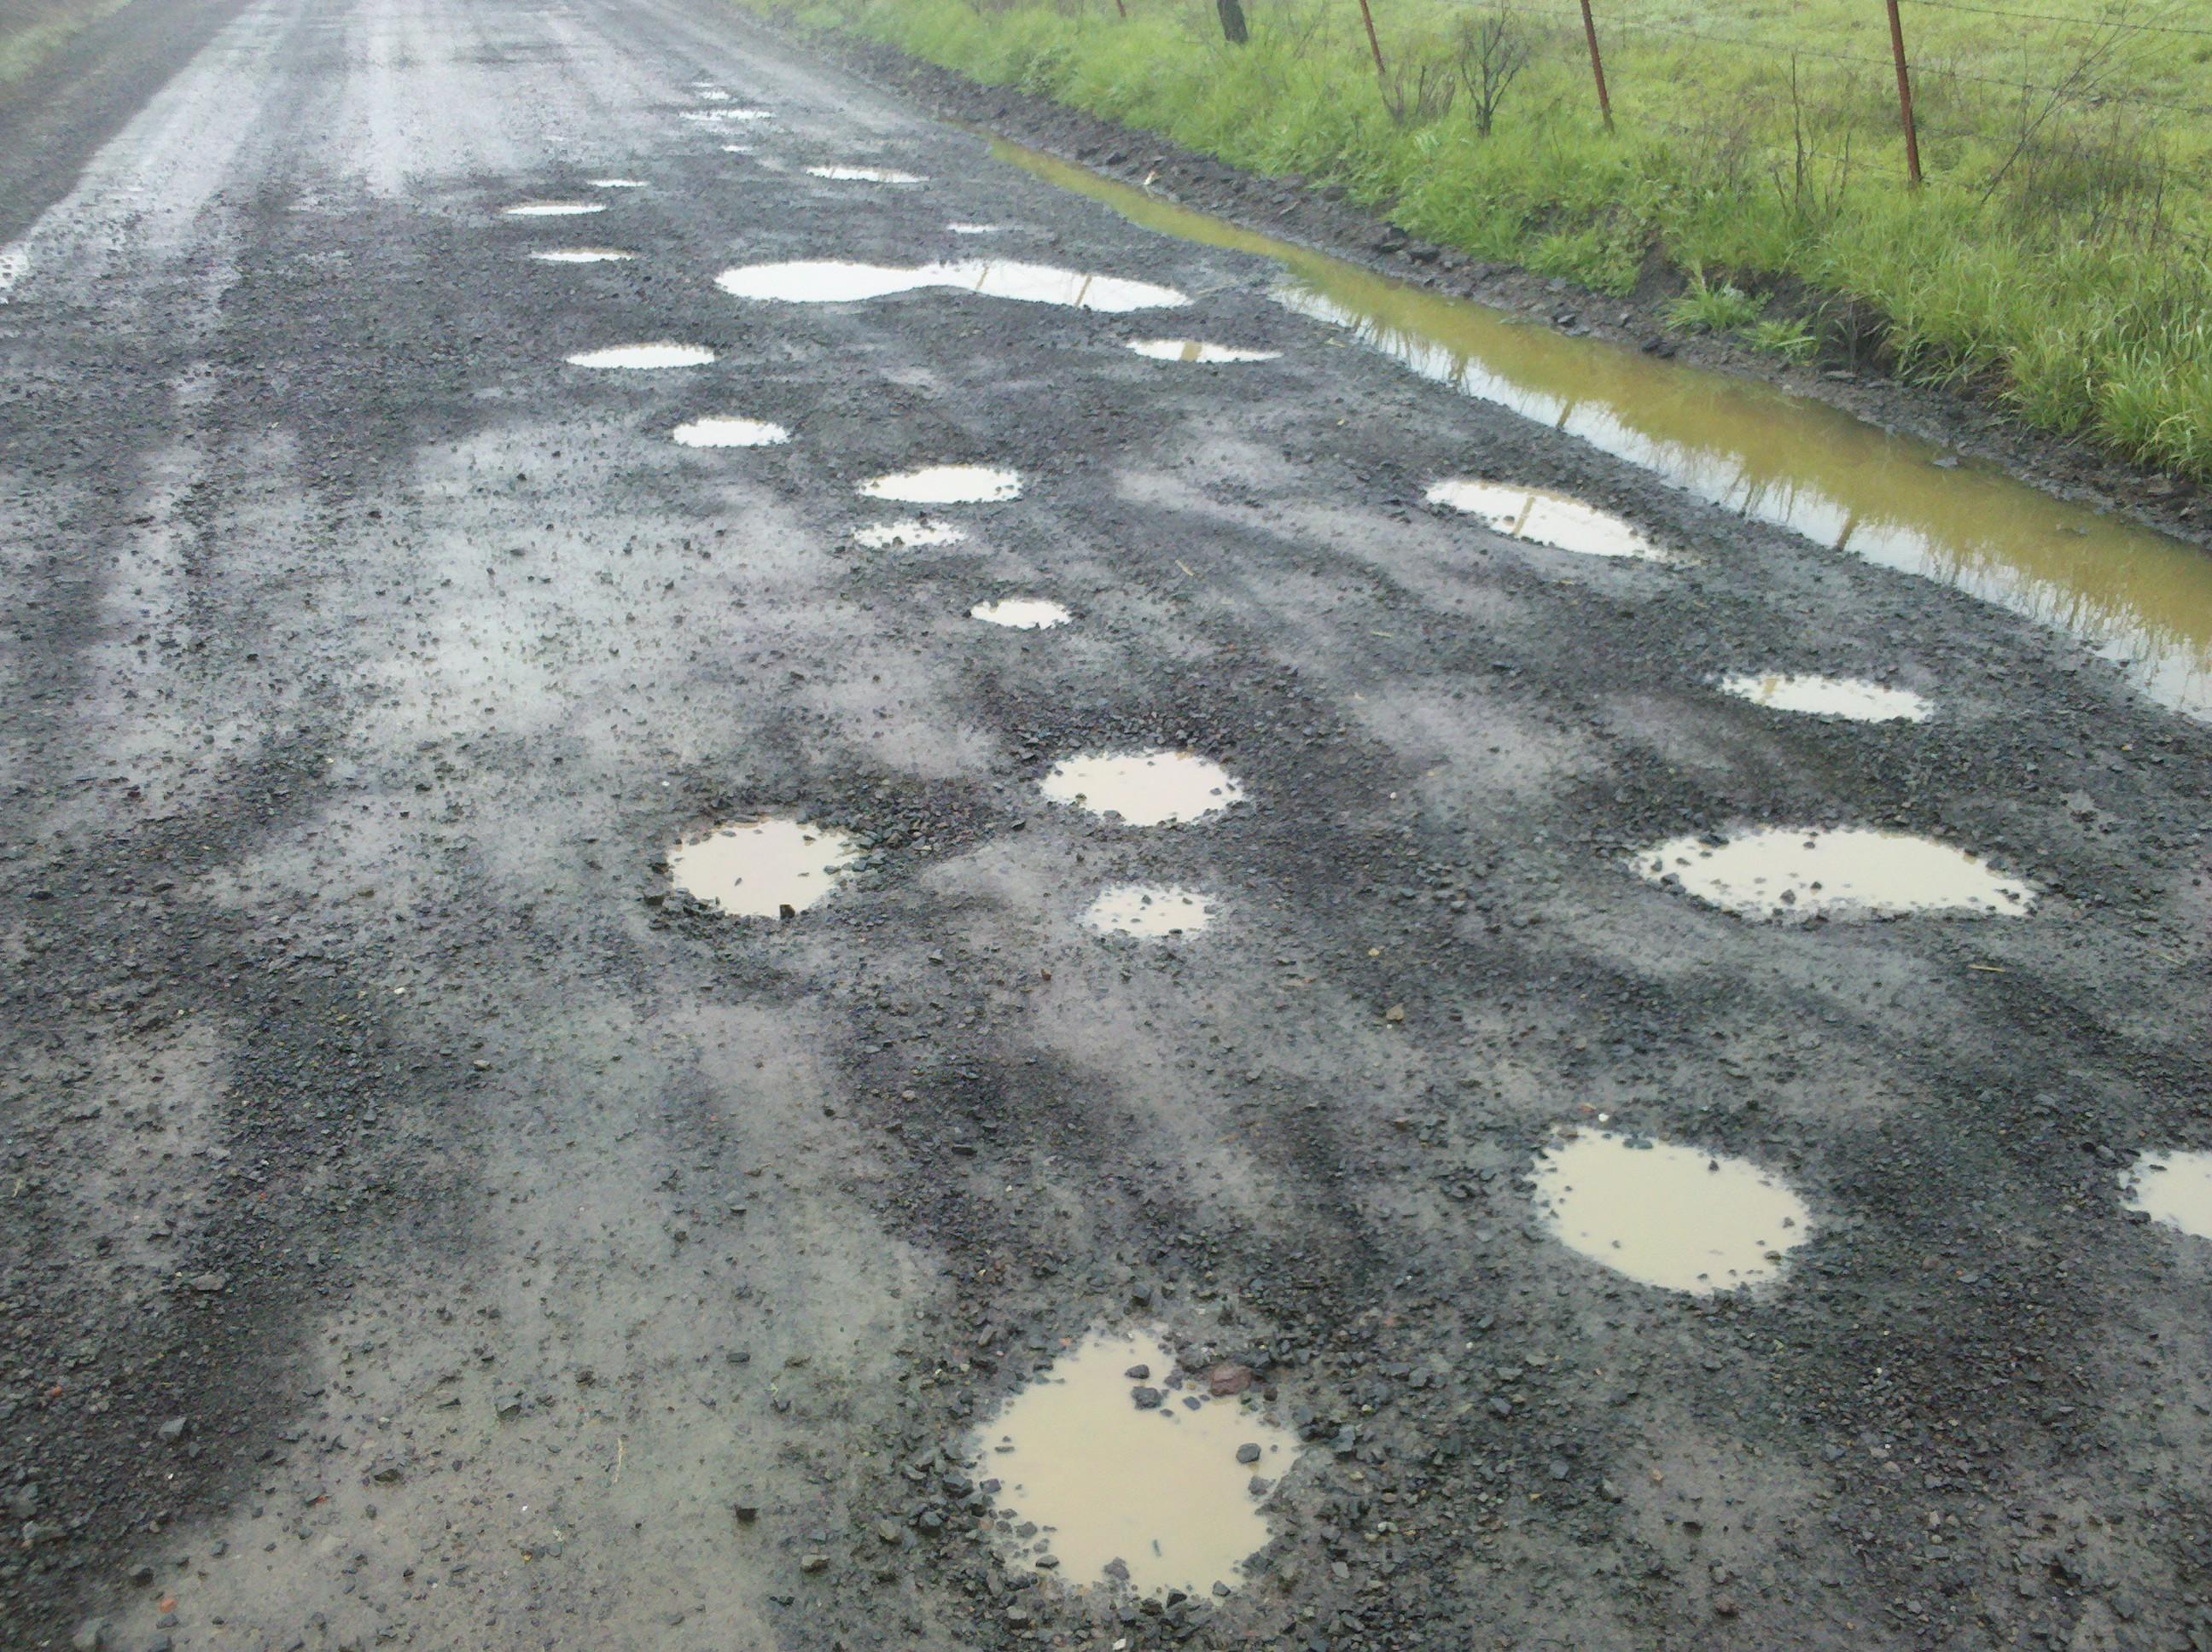
\includegraphics[width = 3in]{images/road_11.jpg}
        \caption{Original Image from the Google Images Dataset}
    \end{figure}

    \begin{figure}[ht!]
        \centering
        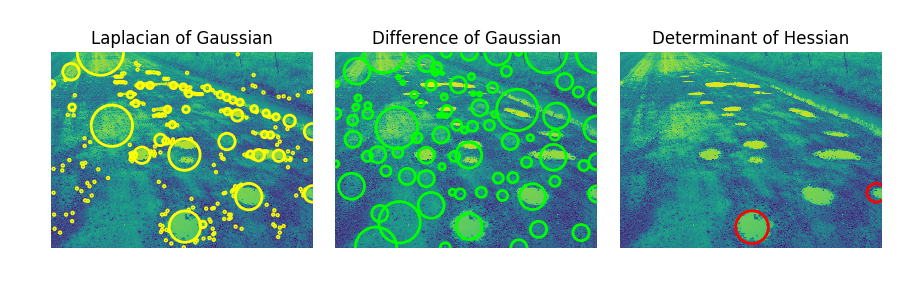
\includegraphics[width = 6in]{images/blob_3.png}
        \caption{Output of the three Blob Detection Techniques}
    \end{figure}
    
    \pagebreak
    
    \begin{figure}[ht!]
        \centering
        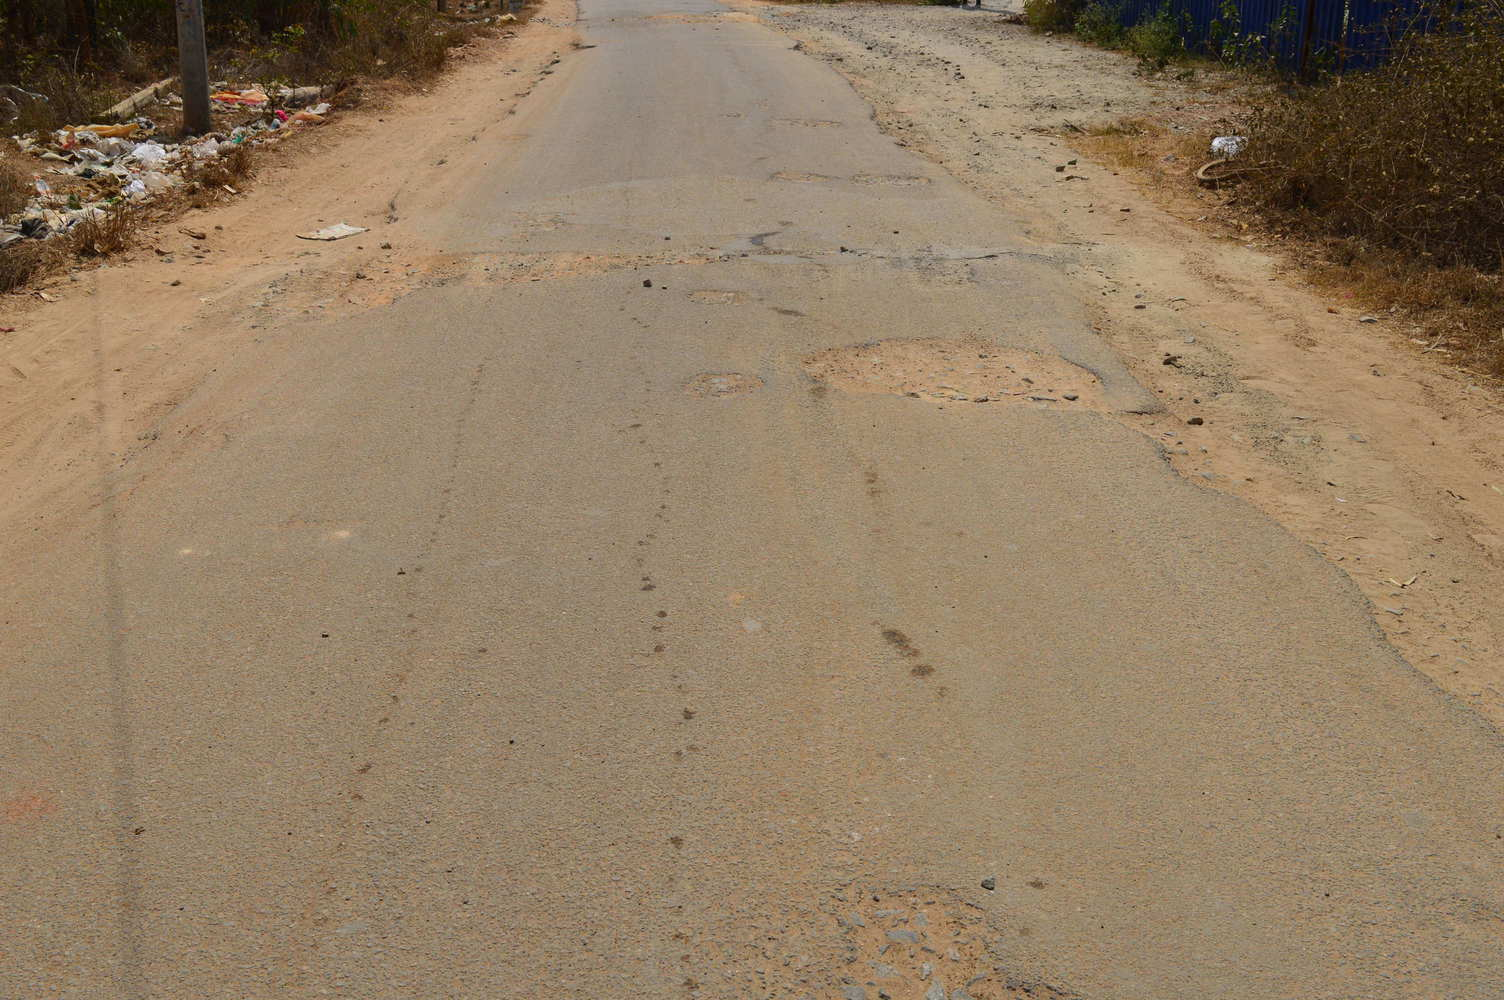
\includegraphics[width = 3in]{images/road_cam_8.jpg}
        \caption{Original Image from the Collected Dataset}
    \end{figure}
    
    \begin{figure}[ht!]
        \centering
        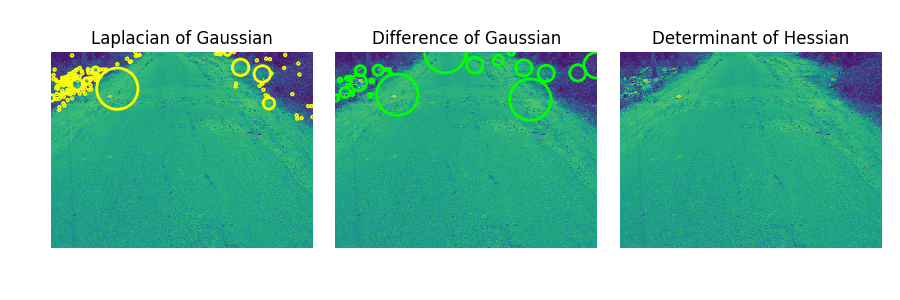
\includegraphics[width = 6in]{images/blob_1.png}
        \caption{Output of the three Blob Detection Techniques}
    \end{figure}
    
    \pagebreak
%    \begin{figure}[ht!]
%        \centering
%        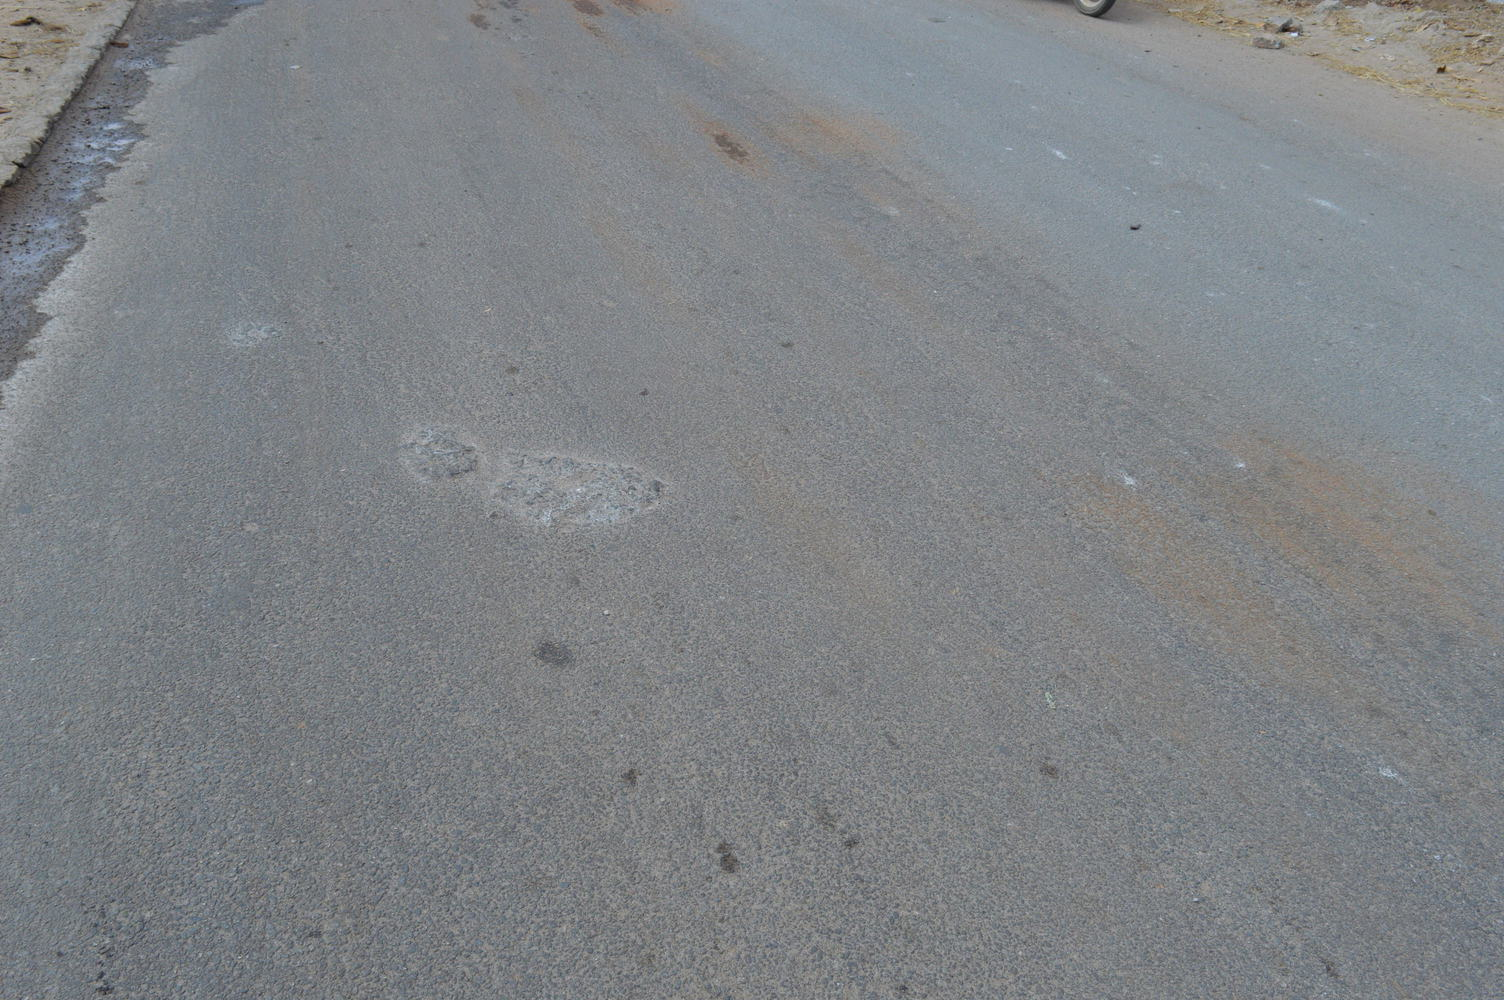
\includegraphics[width = 3in]{images/road_cam_3.jpg}
%        \caption{Original Image from the Collected Dataset}
%    \end{figure}
%
%    \begin{figure}[ht!]
%        \centering
%        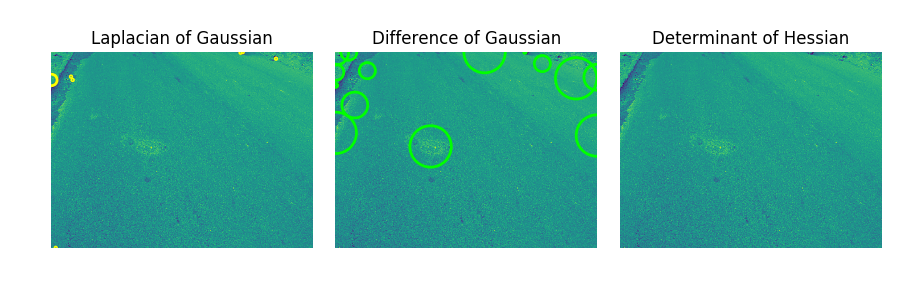
\includegraphics[width = 5in]{images/blob_2.png}
%        \caption{Output of the three Blob Detection Techniques}
%    \end{figure}
%    \pagebreak
    
\item Contour Detection with K-Means \\

In the contour detection method with K-Means, we used the K-Means algorithm with 30 iterations and 3 clusters. The Gaussian Blur was applied to the output of the K-Means to remove any noise in the frames. Finally, the Canny Edge Detection algorithm was used to find out the edges and contours around potholes in the frames. This technique detected potholes and some of the noise in the Google Images dataset but it did not work with our dataset. It missed the contours for potholes and detected shadows in some of the frames.


\begin{figure}[ht!]
        \centering
        \includegraphics[width = 3in]{images/road_7.jpg}
        \caption{Original Image from the Google Images Dataset}
    \end{figure}

    \begin{figure}[ht!]
        \centering
        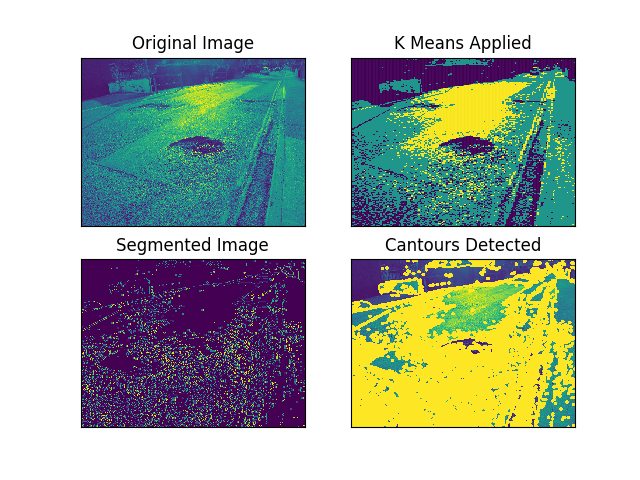
\includegraphics[width = 5in]{images/kmeans_1.png}
        \caption{Output of Contour Detection using K-Means}
    \end{figure}
    \pagebreak
    
    \begin{figure}[ht!]
        \centering
        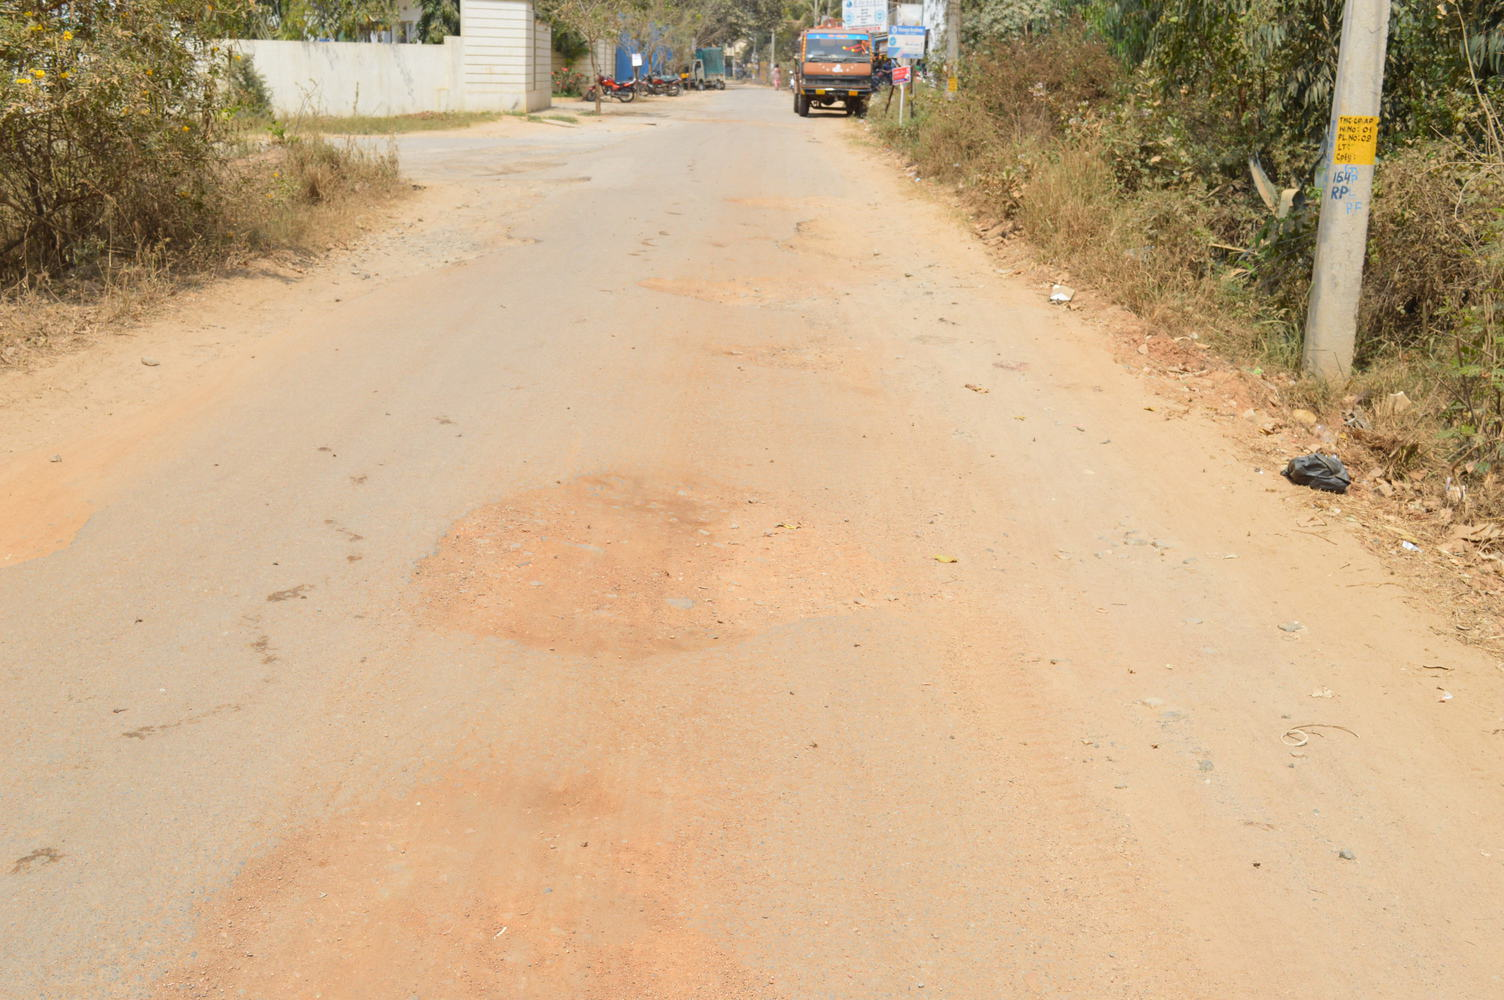
\includegraphics[width = 3in]{images/road_cam_14.jpg}
        \caption{Original Image from the Collected Dataset}
    \end{figure}

    \begin{figure}[ht!]
        \centering
        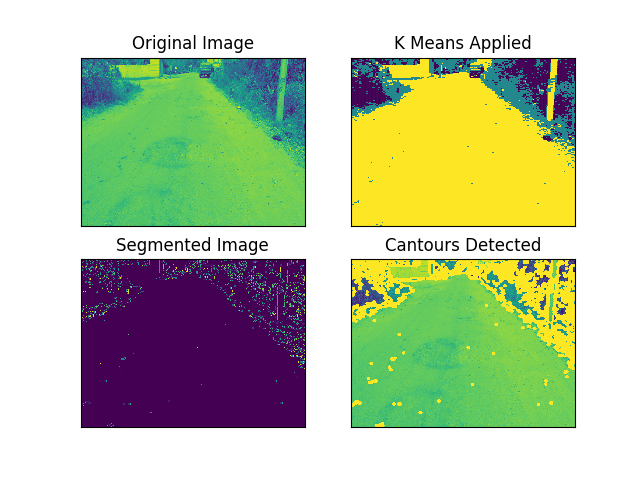
\includegraphics[width = 5in]{images/kmeans_2.png}
        \caption{Output of Contour Detection using K-Means}
    \end{figure}
    \pagebreak
    
    \begin{figure}[ht!]
        \centering
        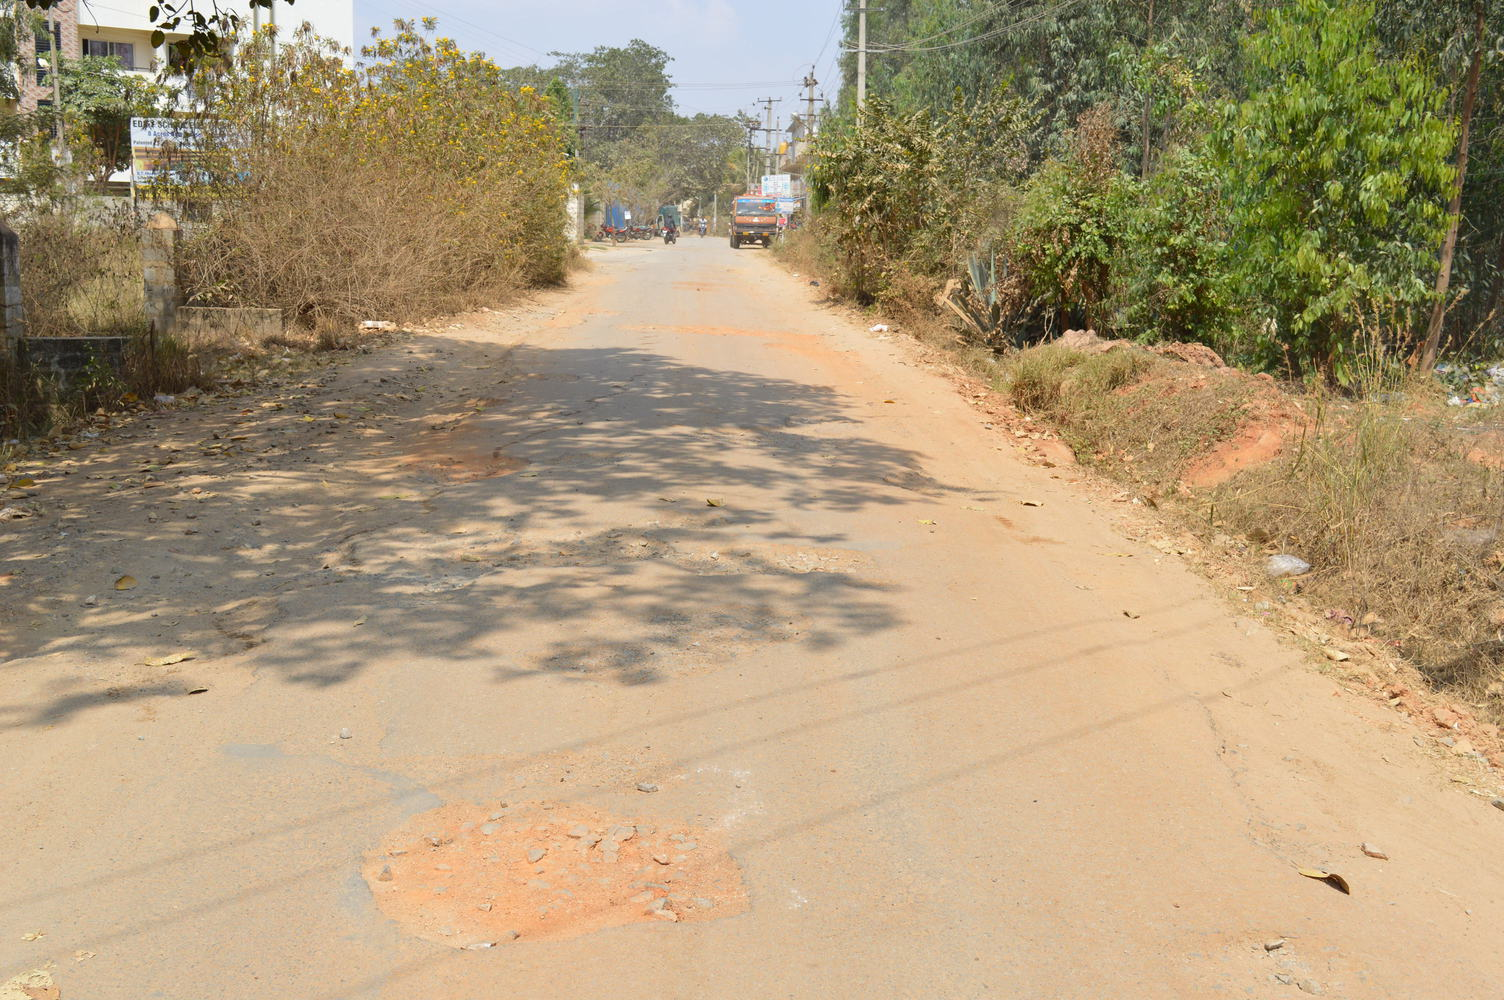
\includegraphics[width = 3in]{images/road_cam_11.jpg}
        \caption{Original Image from the Collected Dataset}
    \end{figure}

    \begin{figure}[ht!]
        \centering
        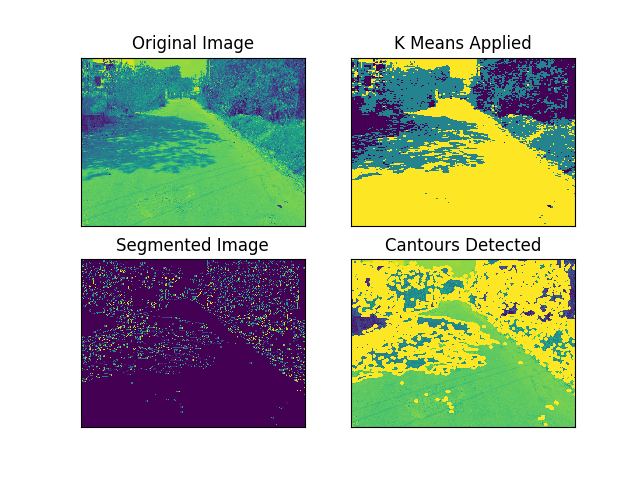
\includegraphics[width = 5in]{images/kmeans_3.png}
        \caption{Output of Contour Detection using K-Means}
    \end{figure}
    \pagebreak

\item Contour Detection with Meanshift \\

Using the idea of the previous methodology of Contour Detection, we used Meanshift as the clustering algorithm instead of the K-means algorithm. The inbuilt function \textbf{pyrMeanShiftFiltering} was used to filter and segment the image with arguments \textbf{Spatial Window Radius} as 25, \textbf{Color Window Radius} as 45 and \textbf{Maximum Level Of Segmentation} as 10. Similar to the previous methodology, Gaussian Blur and Canny Edge Detection were applied to find the contours in the frames.This method worked perfectly on the Google Images Dataset but detected the potholes partially in our dataset with the additional noise.

    \begin{figure}[ht!]
        \centering
        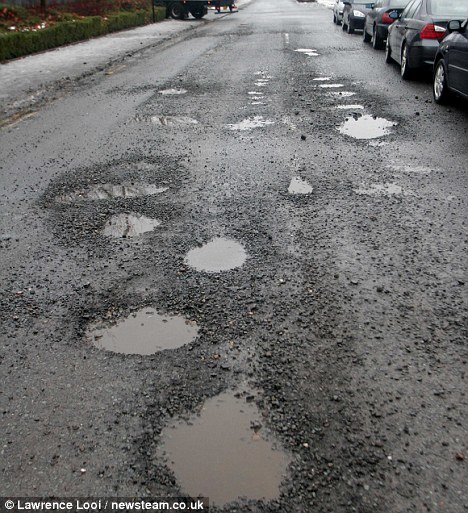
\includegraphics[width = 2in]{images/road_10.jpg}
        \caption{Original Image from the Google Images Dataset}
    \end{figure}

    \begin{figure}[ht!]
        \centering
        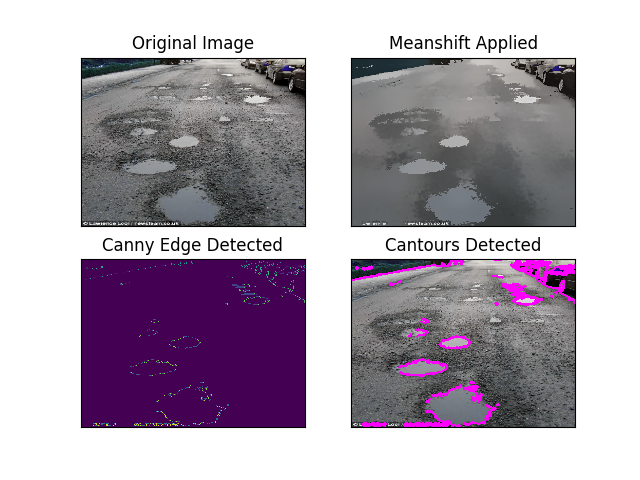
\includegraphics[width = 5in]{images/meanshift_2.png}
        \caption{Output of Contour Detection using Meanshift}
    \end{figure}
    \pagebreak
    
    \begin{figure}[ht!]
        \centering
        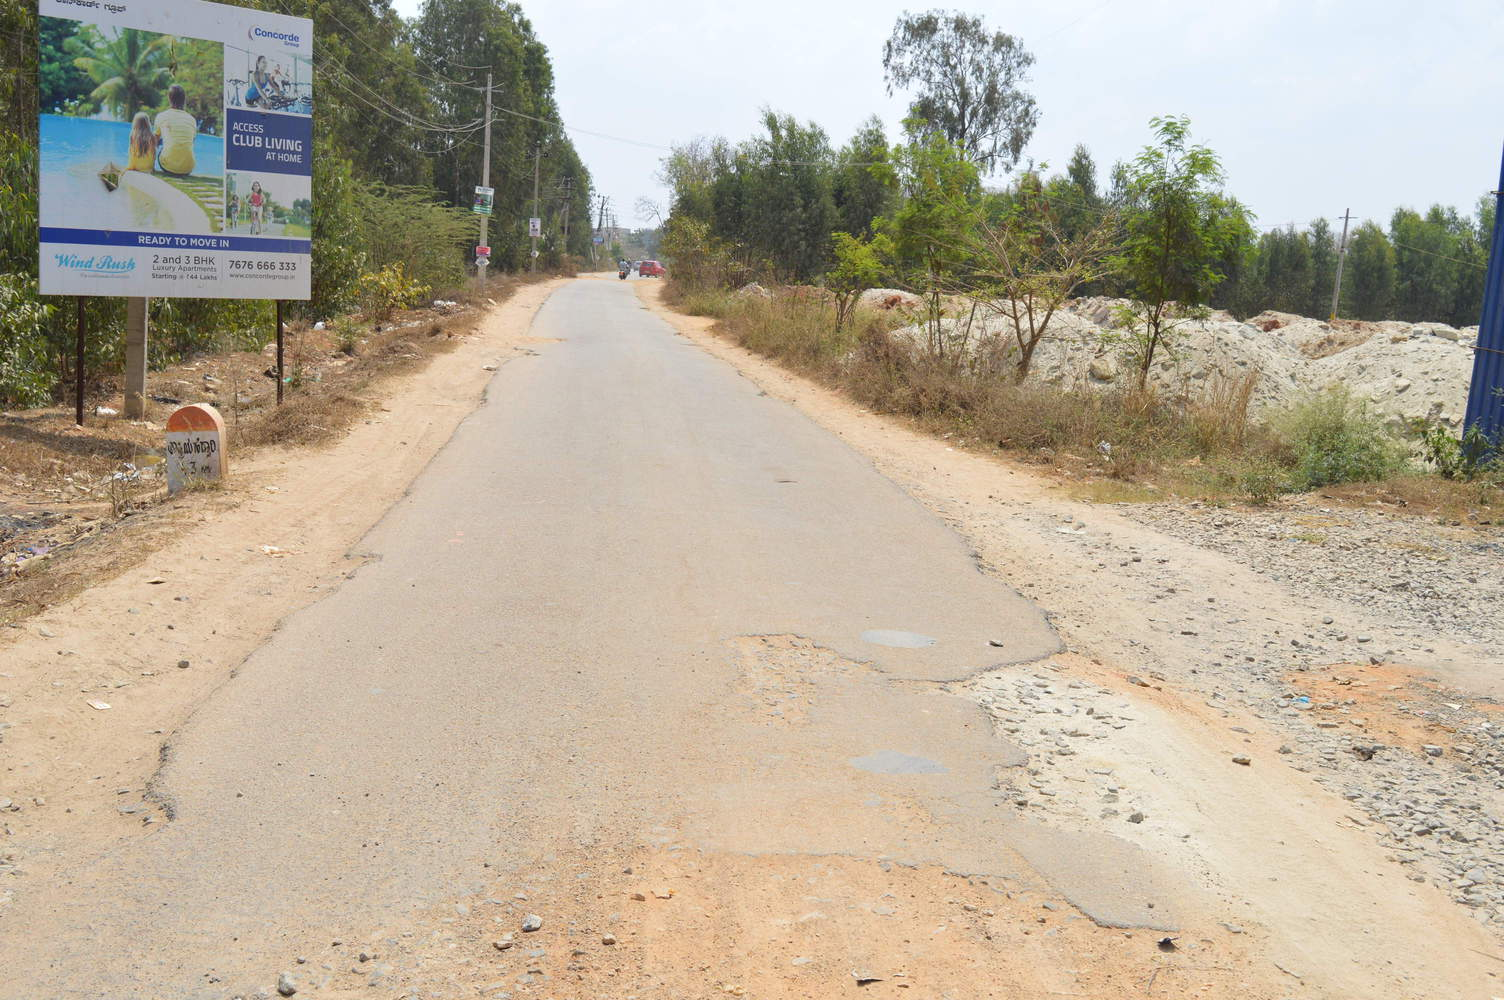
\includegraphics[width = 3in]{images/road_cam_25.jpg}
        \caption{Original Image from the Collected Dataset}
    \end{figure}

    \begin{figure}[ht!]
        \centering
        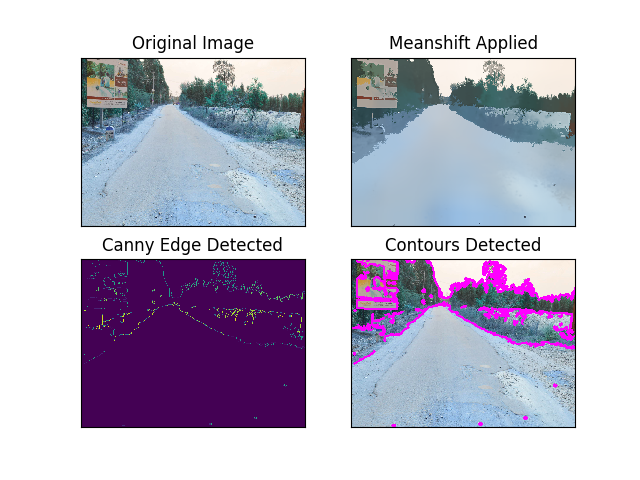
\includegraphics[width = 5in]{images/meanshift_1.png}
        \caption{Output of Contour Detection using Meanshift}
    \end{figure}
    \pagebreak

    
    \begin{figure}[ht!]
        \centering
        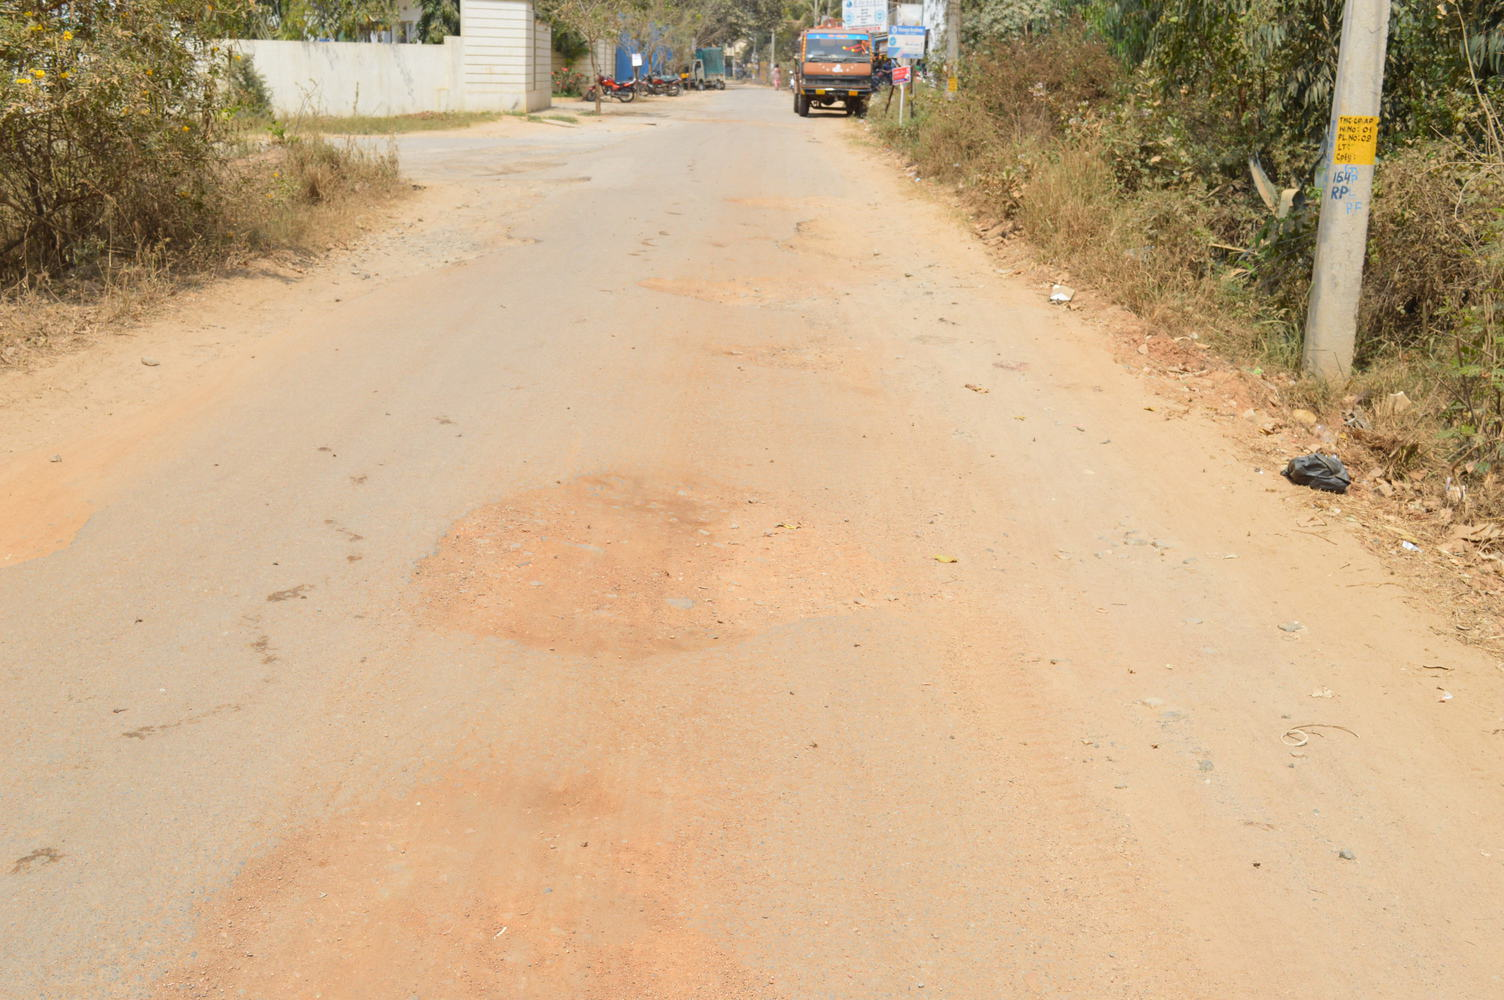
\includegraphics[width = 3in]{images/road_cam_14.jpg}
        \caption{Original Image from the Collected Dataset}
    \end{figure}

    \begin{figure}[ht!]
        \centering
        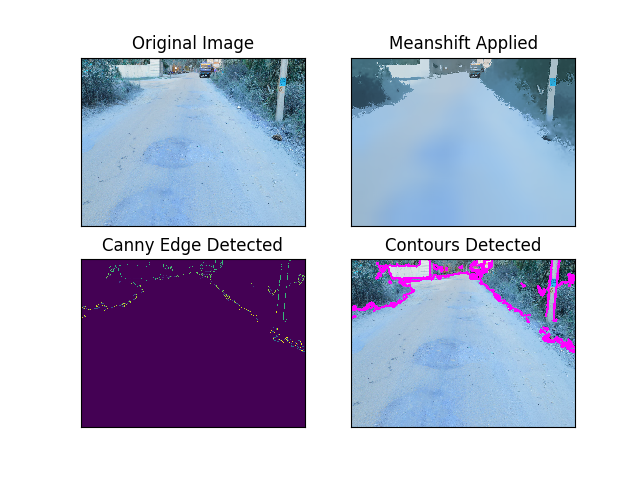
\includegraphics[width = 5in]{images/meanshift_3.png}
        \caption{Output of Contour Detection using Meanshift}
    \end{figure}
    \pagebreak
    
    \begin{figure}[ht!]
        \centering
        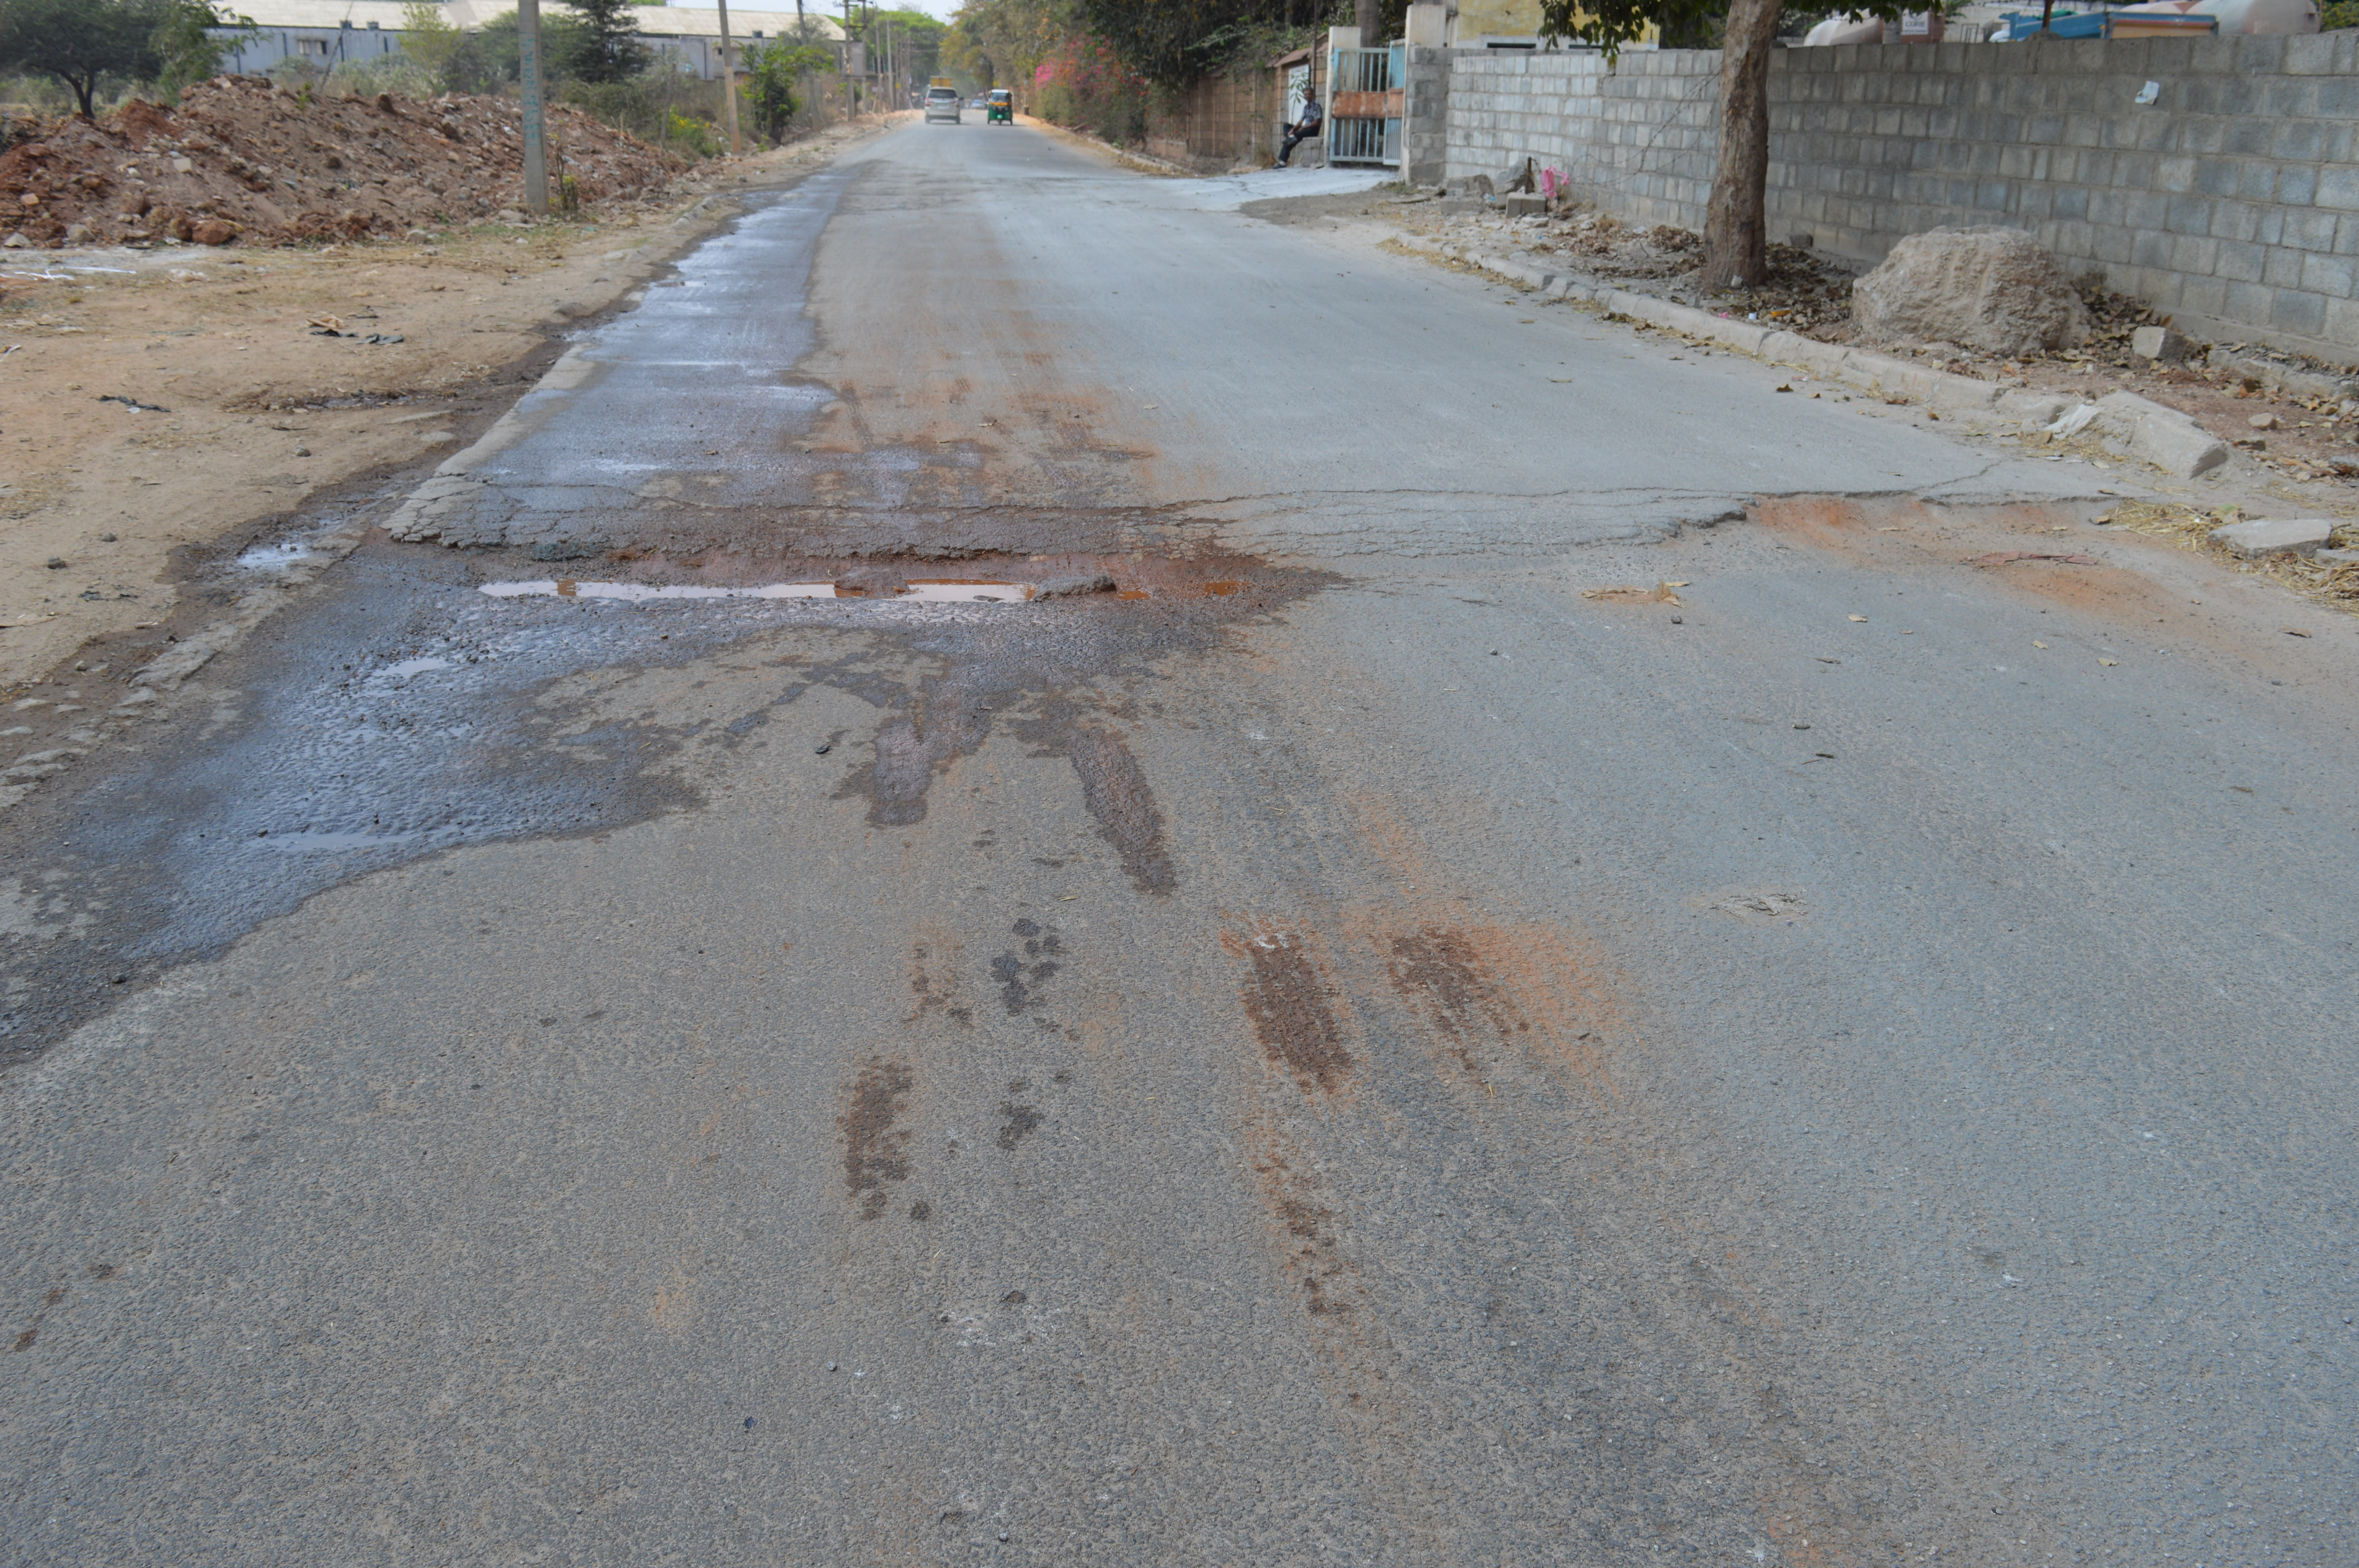
\includegraphics[width = 3in]{images/DSC_2524.JPG}
        \caption{Original Image from the Collected Dataset}
    \end{figure}

    \begin{figure}[ht!]
        \centering
        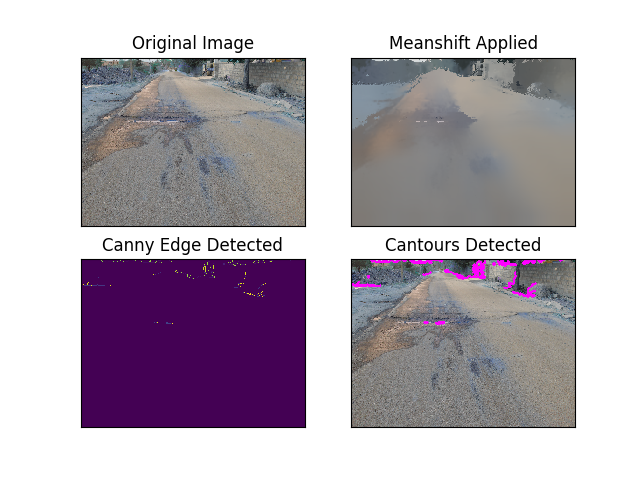
\includegraphics[width = 5in]{images/meanshift_4.png}
        \caption{Output of Contour Detection using Meanshift}
    \end{figure}
    \pagebreak

\newpage
    
\item Contour Detection with Morphological Transformation \\

In the Contour Detection method with Morphological Transformations, we used erosion to detect contours around potholes in the images. Gaussian Blur and thresholding was applied on the input frames to remove the noise signals from the image. The results of Image Gradients: Laplacian, Sobel X, Sobel Y were compared, after applying them on the blurred image. Among all, Sobel Y, performed the best. Then, erosion was applied to this output frame, with the medium sized kernel, to narrow down the search for potholes in the frames. Contours were being detected in the final frame. This technique worked on the Google Images dataset with partial noise being detected but detected too much noise in our dataset along with a fraction of potholes.    

\begin{figure}[ht!]
        \centering
        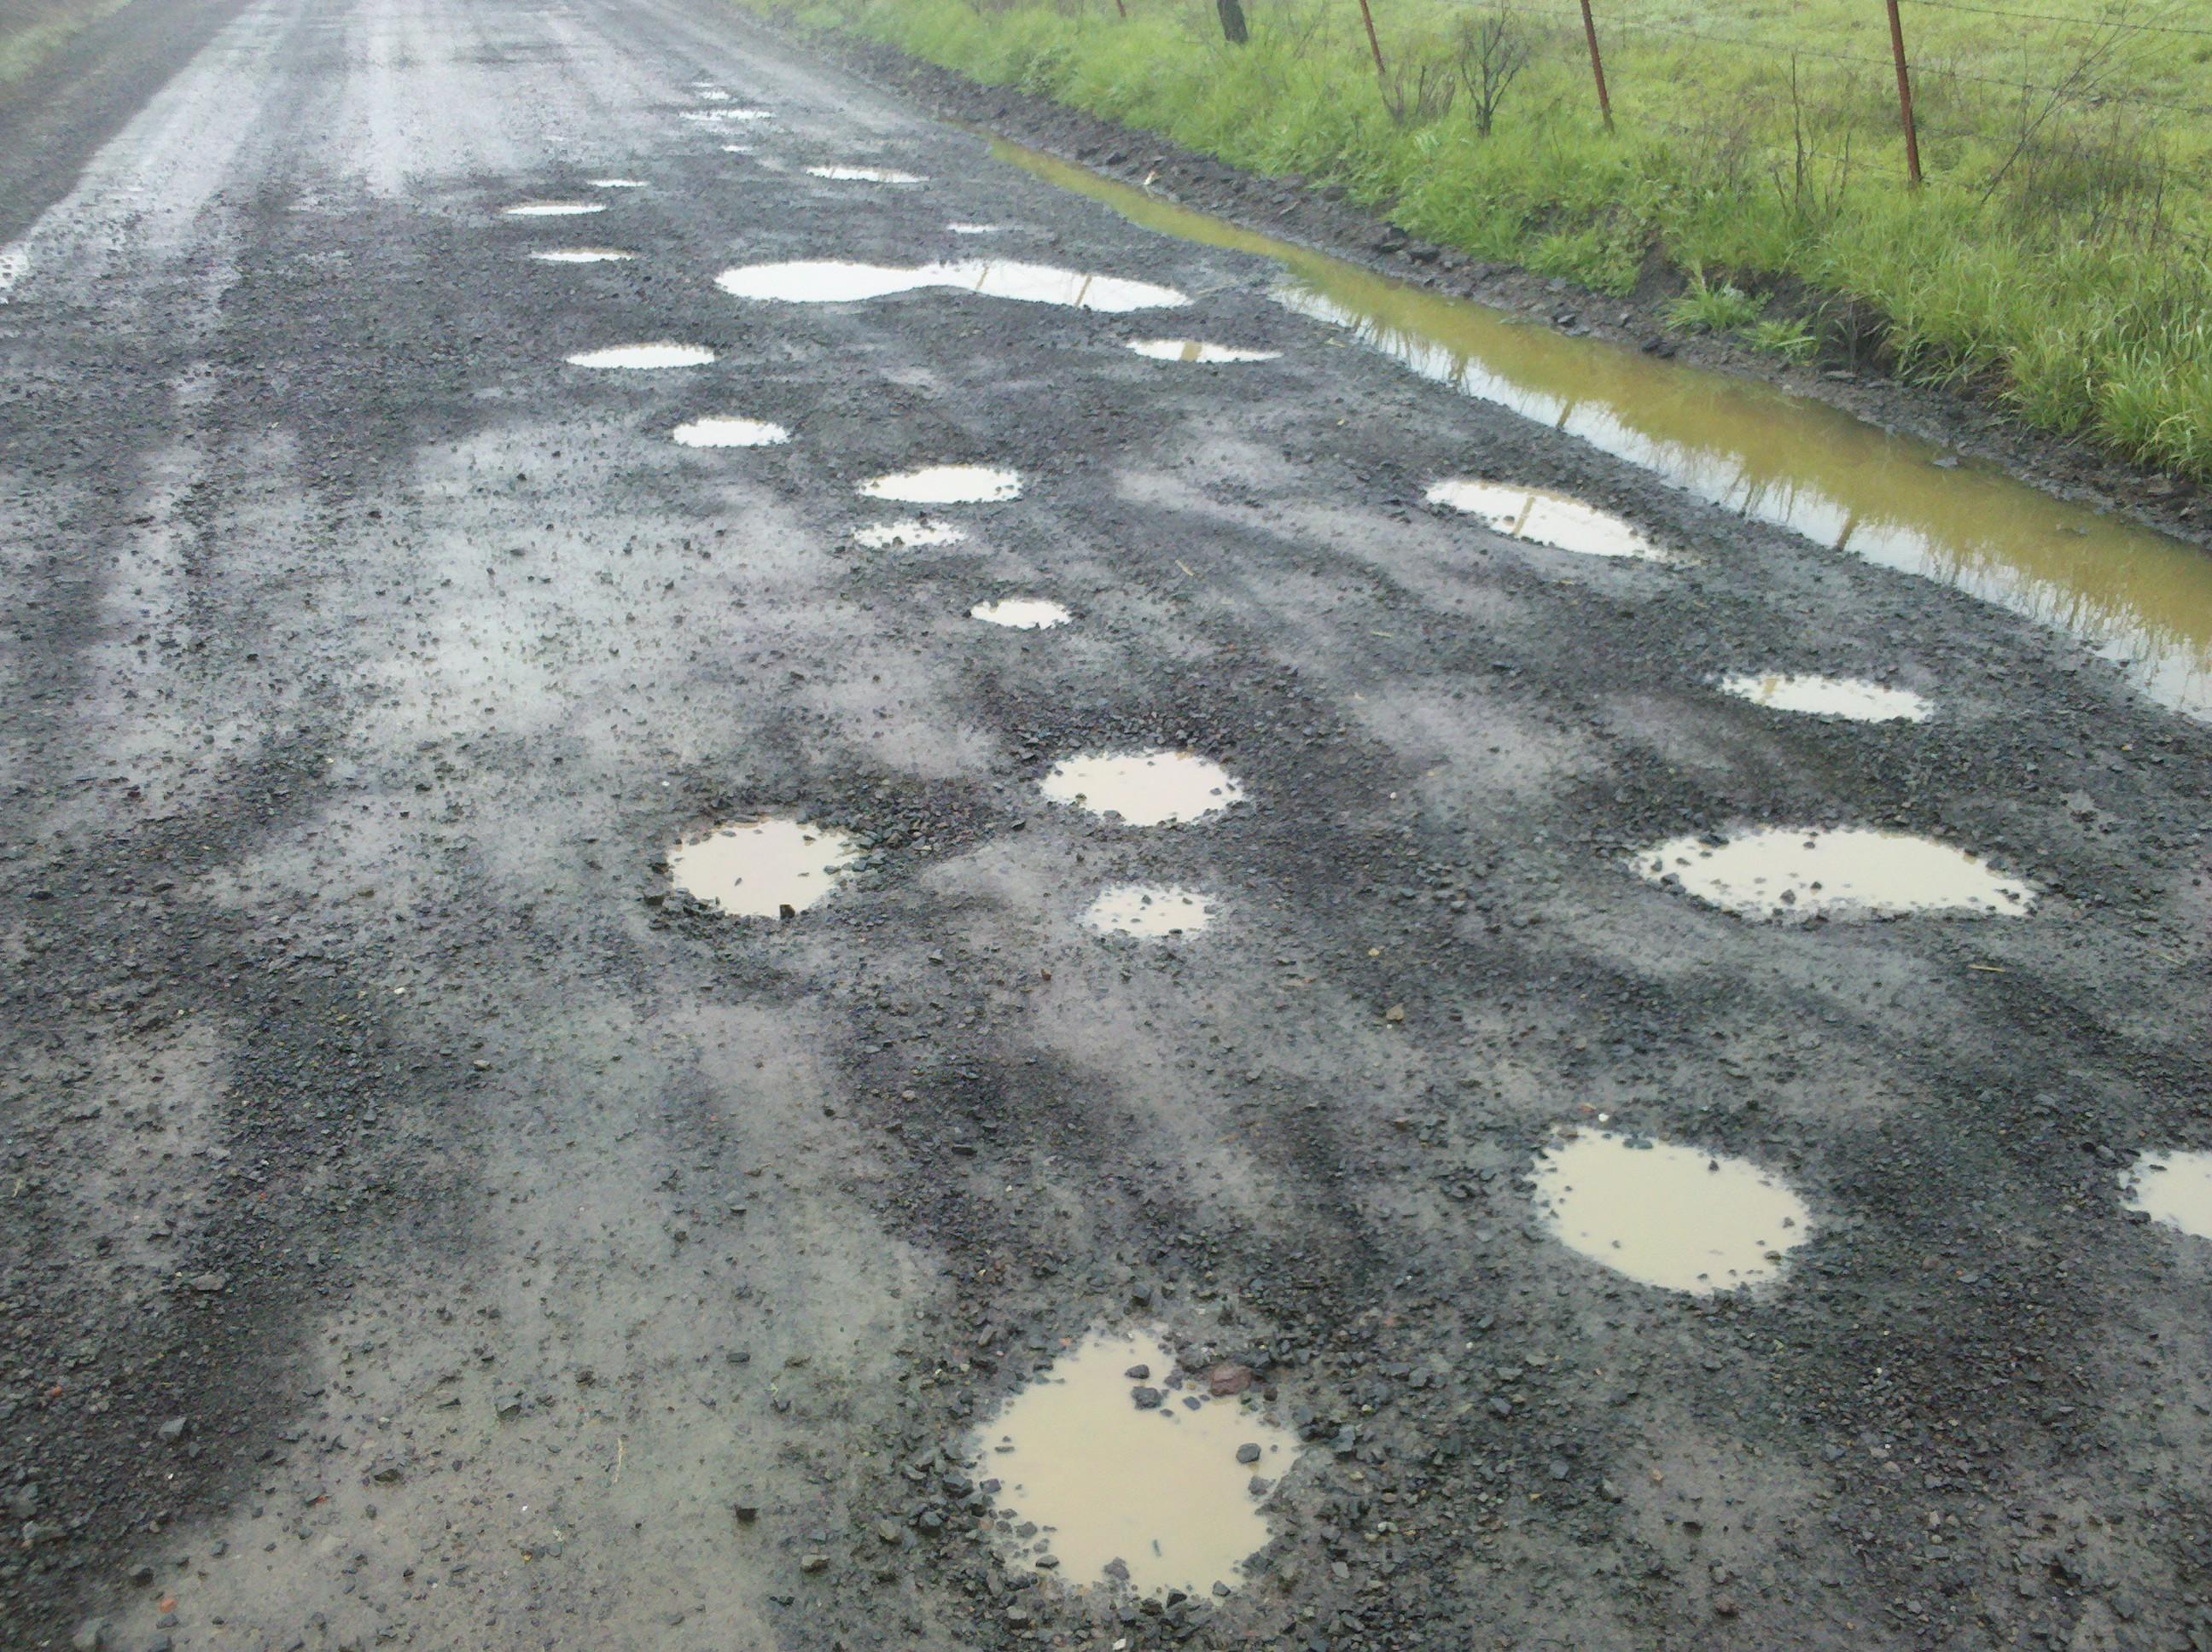
\includegraphics[width = 3in]{images/road_11.jpg}
        \caption{Original Image from the Google Images Dataset}
    \end{figure}

    \begin{figure}[ht!]
        \centering
        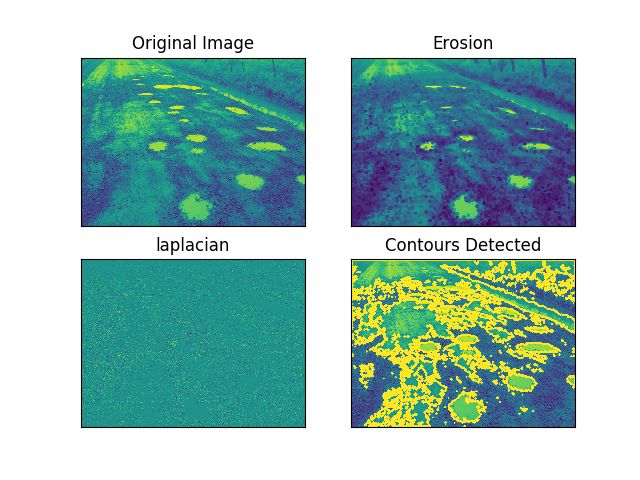
\includegraphics[width = 5in]{images/morph_transform_2.png}
        \caption{Output of Contour Detection using Morphological Transformation}
    \end{figure}
    \pagebreak
    
    \begin{figure}[ht!]
        \centering
        \includegraphics[width = 3in]{images/road_7.jpg}
        \caption{Original Image from the Google Images Dataset}
    \end{figure}

    \begin{figure}[ht!]
        \centering
        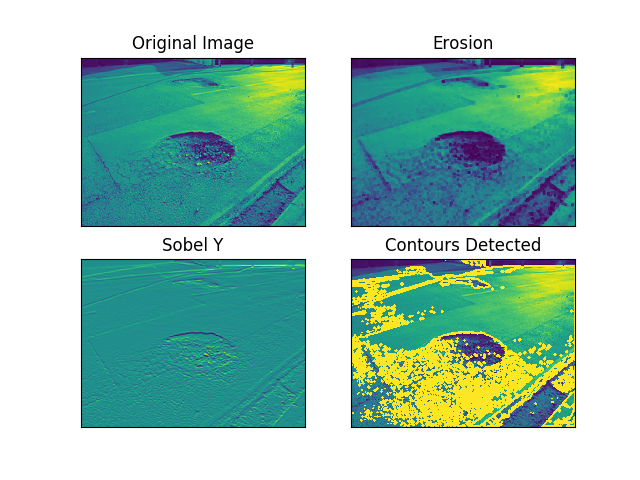
\includegraphics[width = 5in]{images/morph_transform_6.png}
        \caption{Output of Contour Detection using Morphological Transformation}
    \end{figure}
    \pagebreak
    
    \begin{figure}[ht!]
        \centering
        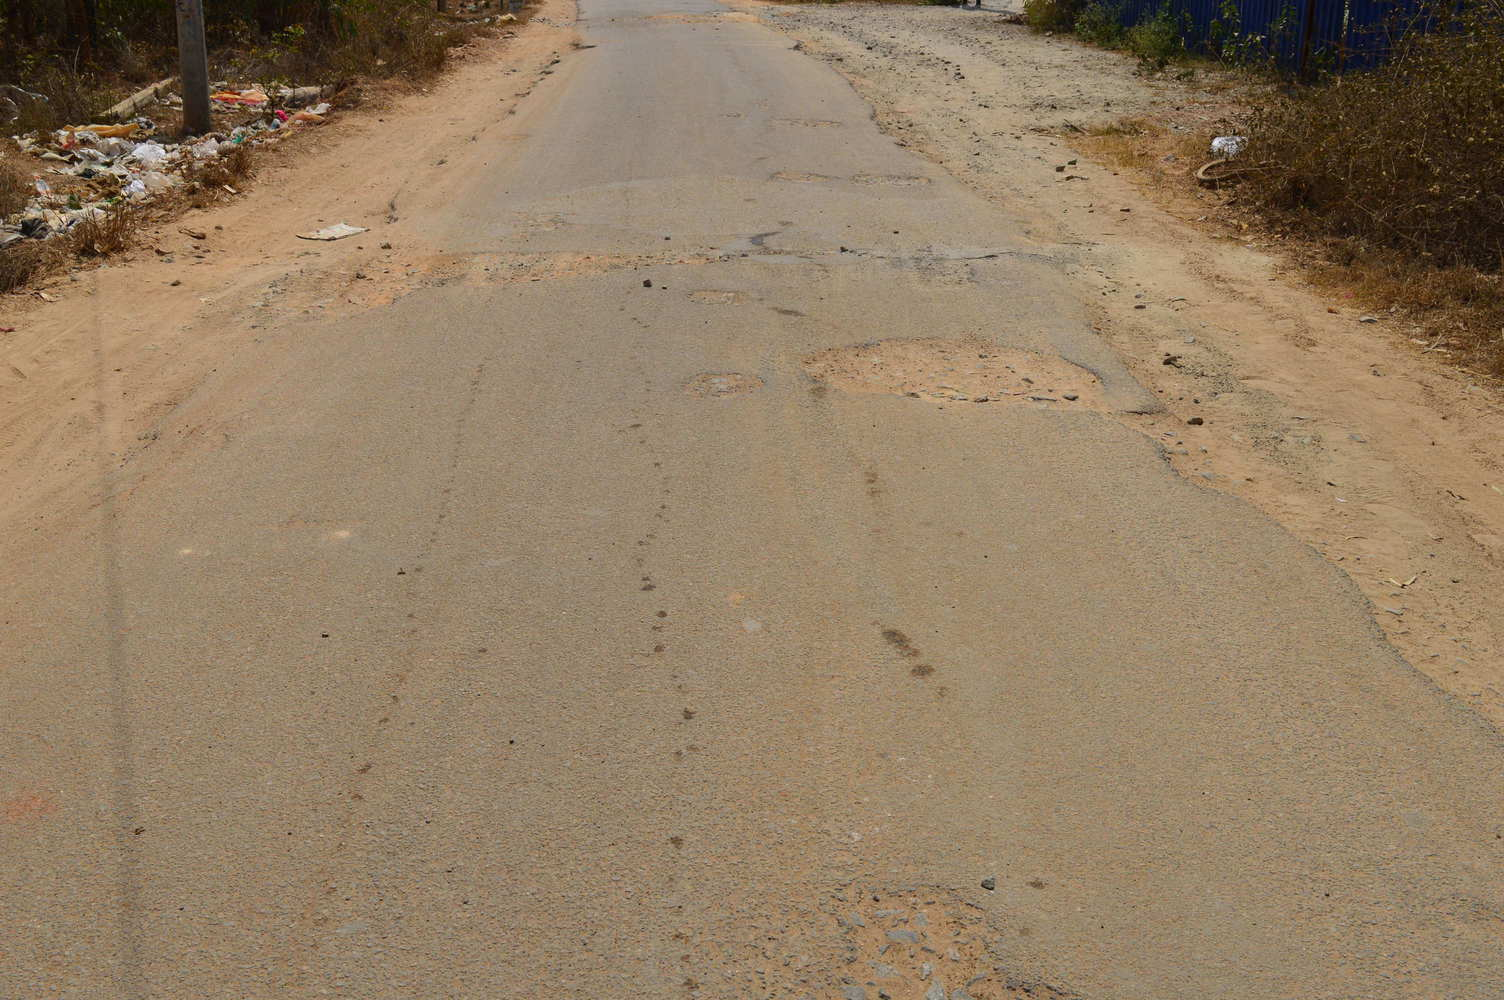
\includegraphics[width = 3in]{images/road_cam_8.jpg}
        \caption{Original Image from the Collected Dataset}
    \end{figure}

    \begin{figure}[ht!]
        \centering
        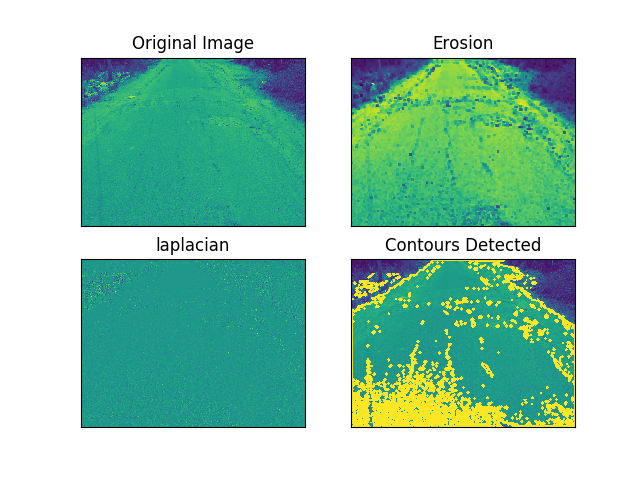
\includegraphics[width = 5in]{images/morph_transform_3.png}
        \caption{Output of Contour Detection using Morphological Transformation}
    \end{figure}
    \pagebreak
    
    \begin{figure}[ht!]
        \centering
        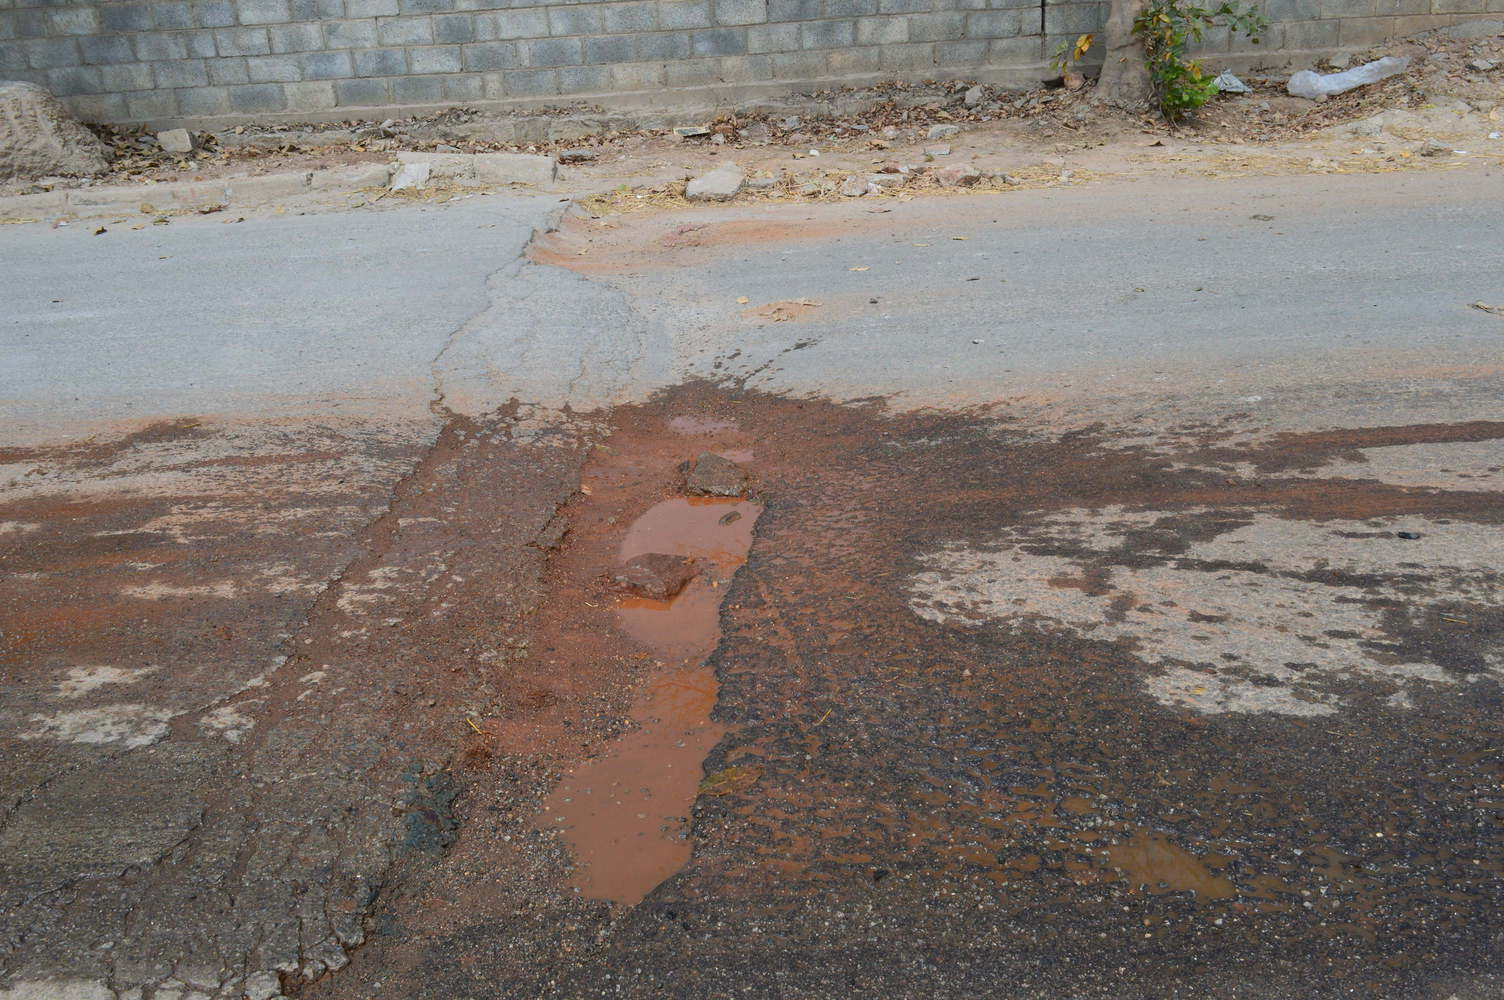
\includegraphics[width = 3in]{images/road_cam_2.jpg}
        \caption{Original Image from the Collected Dataset}
    \end{figure}

    \begin{figure}[ht!]
        \centering
        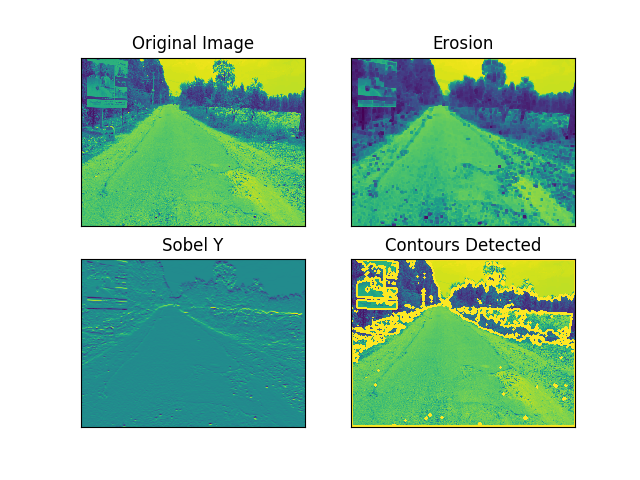
\includegraphics[width = 5in]{images/morph_transform_4.png}
        \caption{Output of Contour Detection using Morphological Transformation}
    \end{figure}
    \pagebreak
    
    \begin{figure}[ht!]
        \centering
        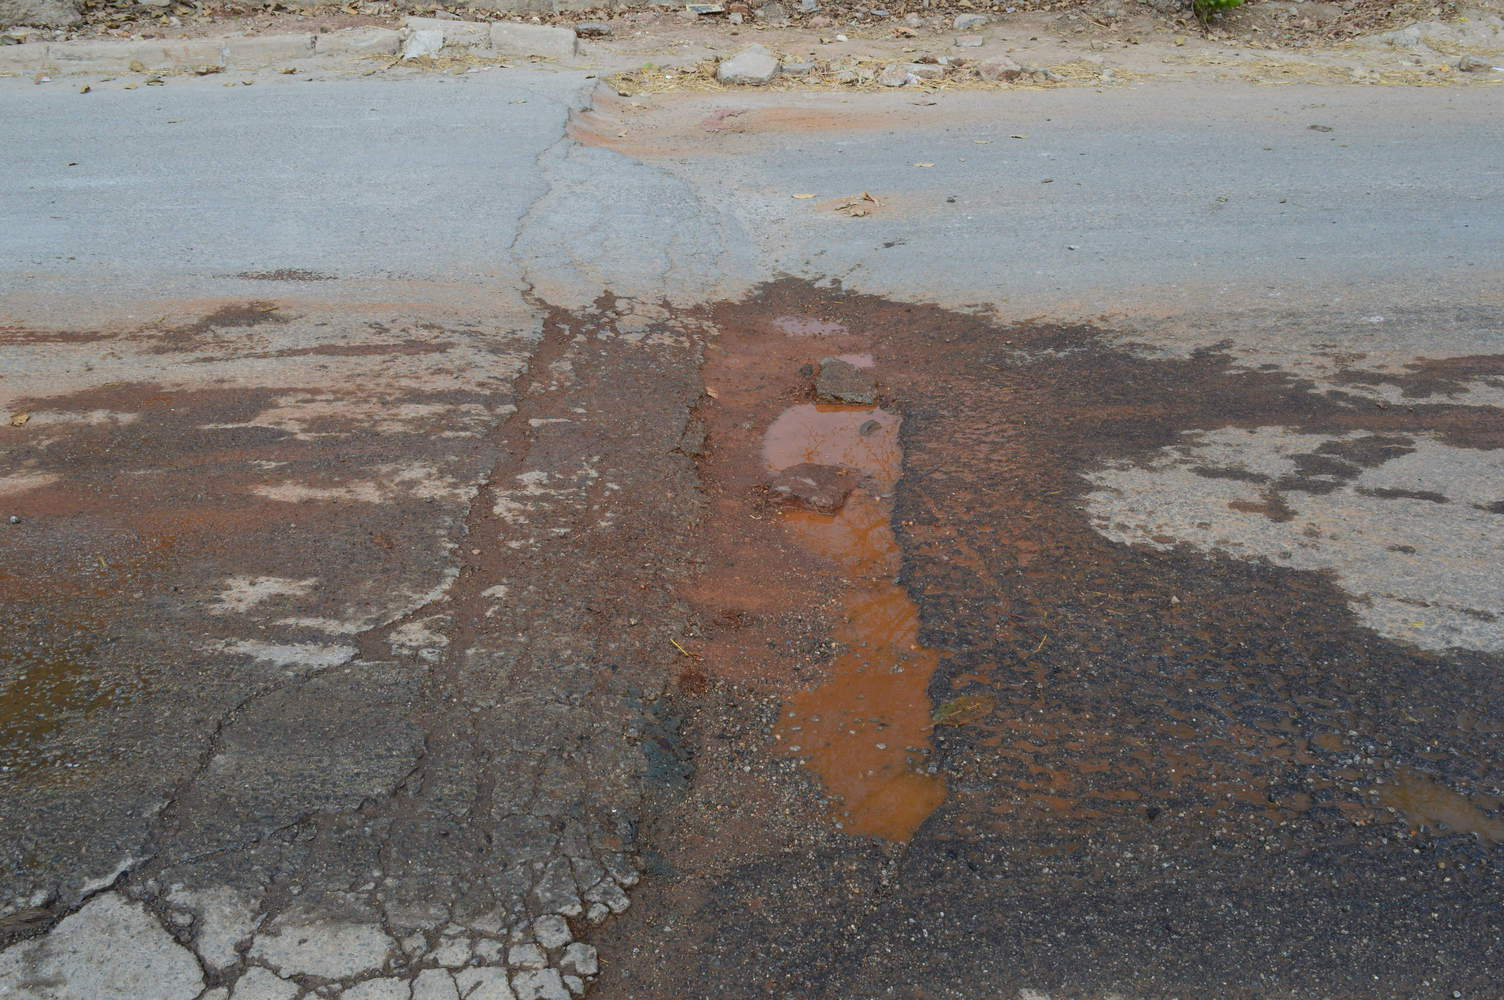
\includegraphics[width = 3in]{images/road_cam_6.jpg}
        \caption{Original Image from the Collected Dataset}
    \end{figure}

    \begin{figure}[ht!]
        \centering
        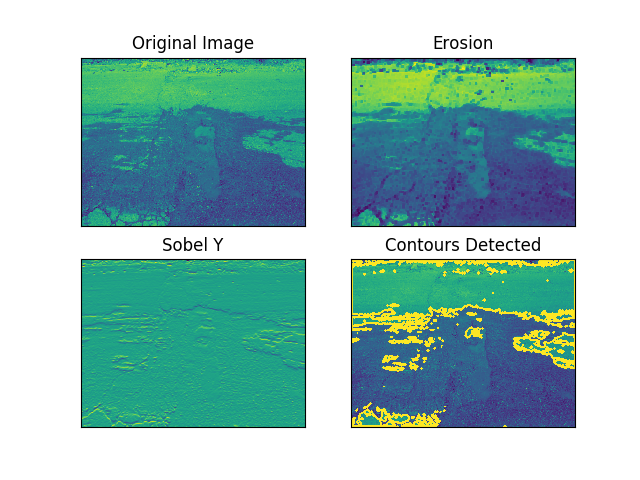
\includegraphics[width = 5in]{images/morph_transform_5.png}
        \caption{Output of Contour Detection using Morphological Transformation}
    \end{figure}
    \pagebreak
    
    \begin{figure}[ht!]
        \centering
        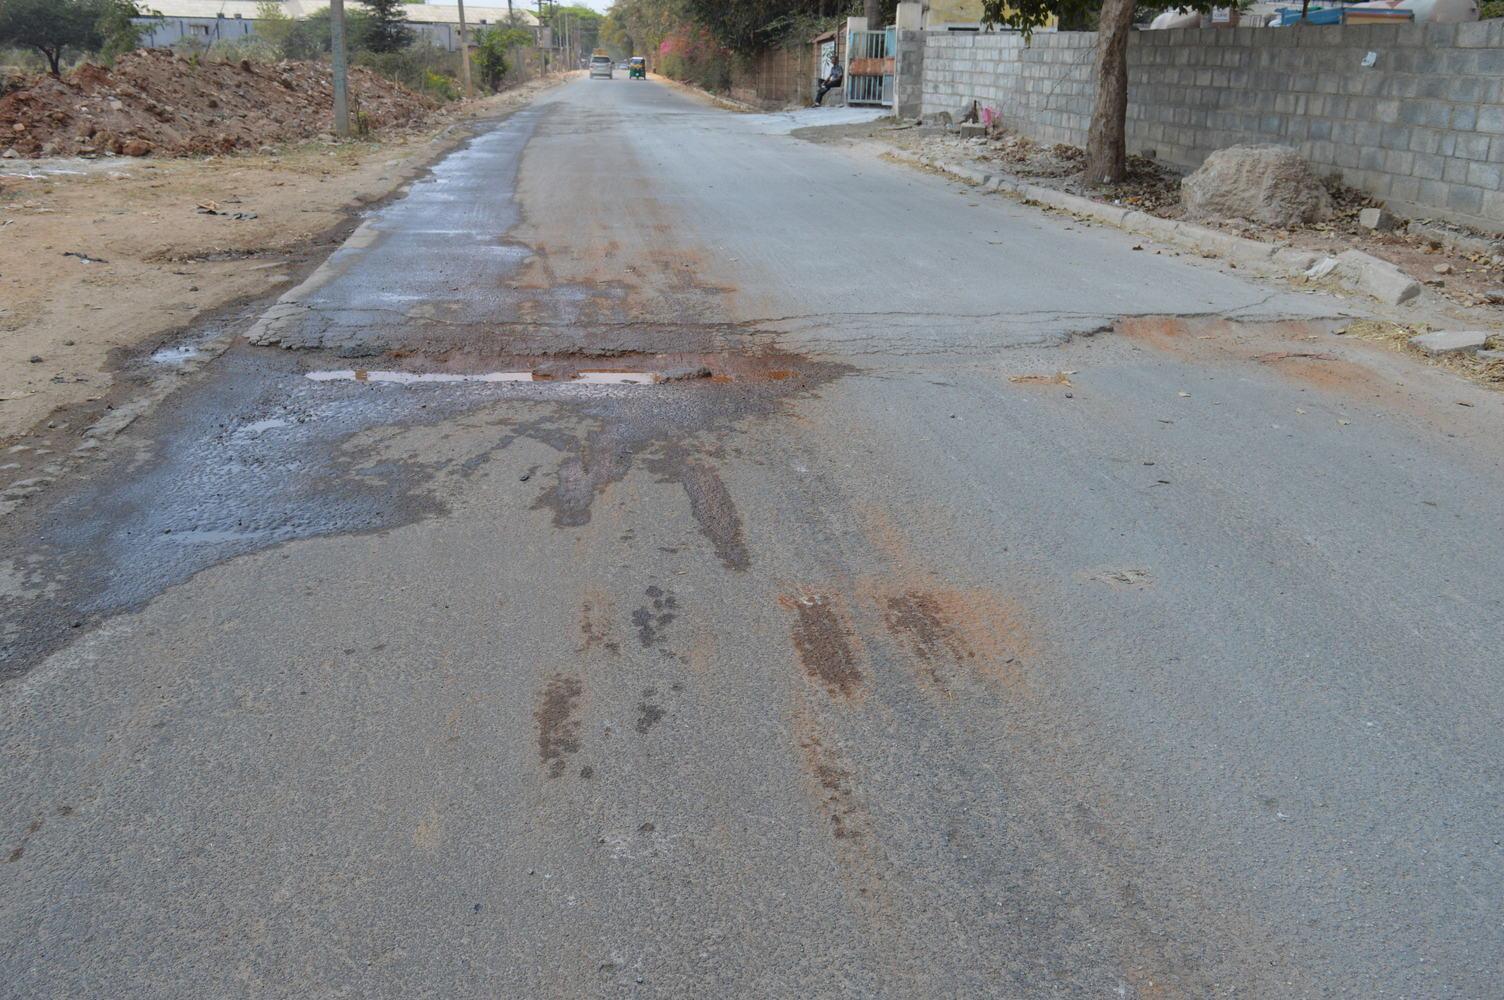
\includegraphics[width = 3in]{images/road_cam_4.jpg}
        \caption{Original Image from the Collected Dataset}
    \end{figure}

    \begin{figure}[ht!]
        \centering
        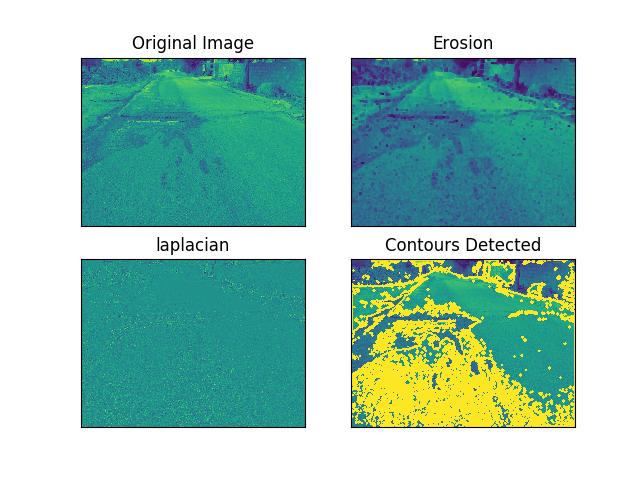
\includegraphics[width = 5in]{images/morph_transform_1.png}
        \caption{Output of Contour Detection using Morphological Transformation}
    \end{figure}
    \pagebreak
    
    \begin{figure}[ht!]
        \centering
        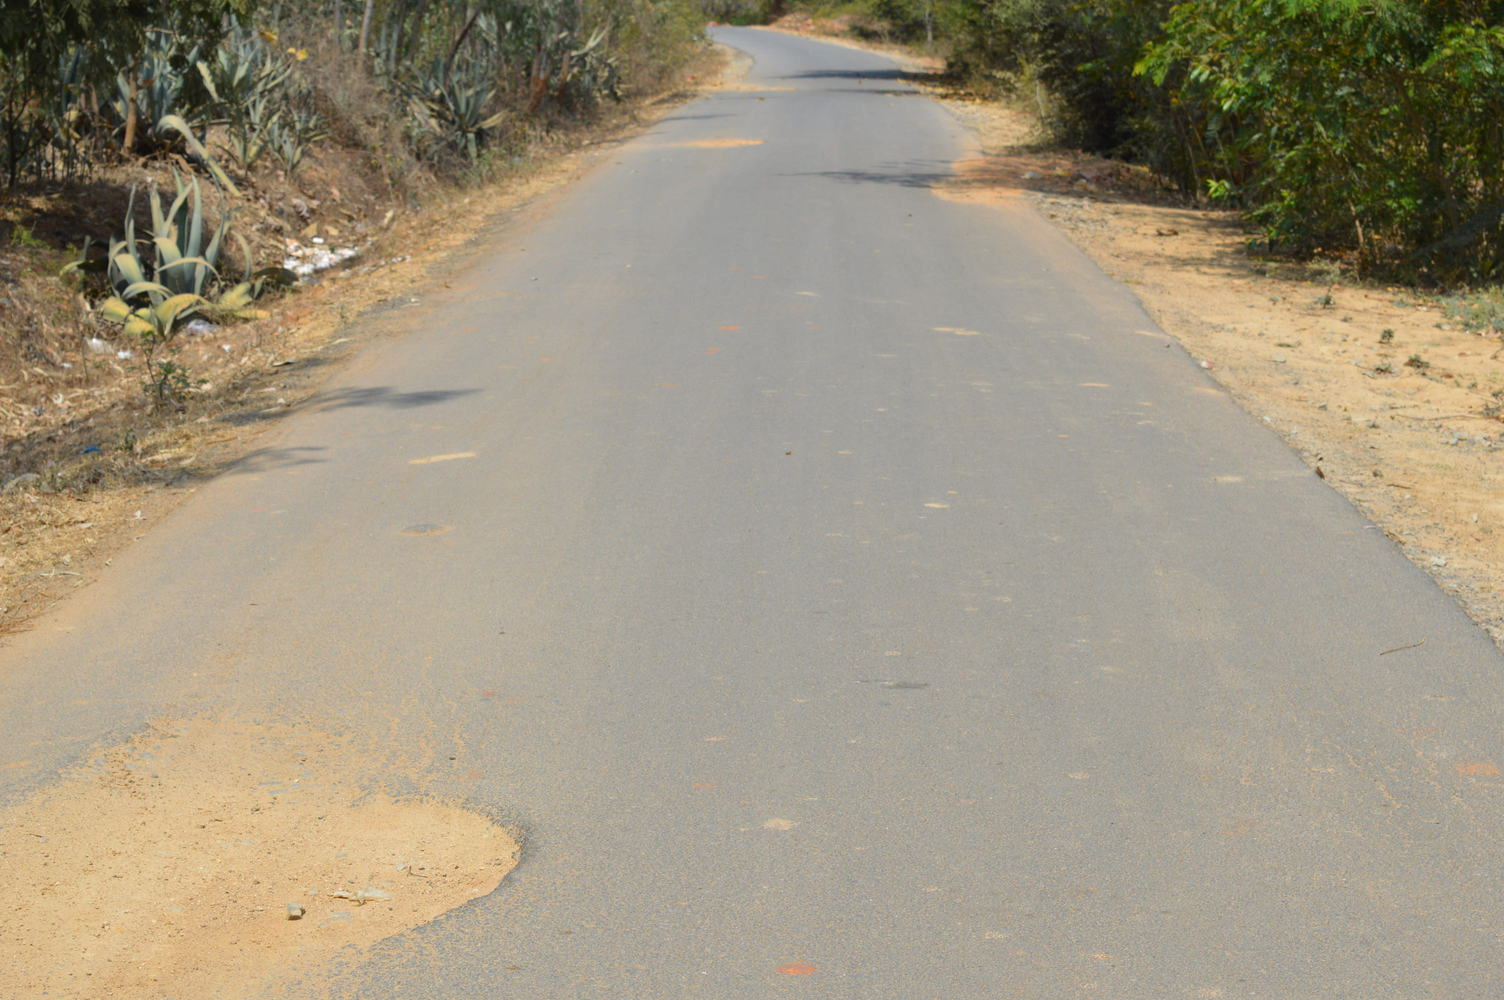
\includegraphics[width = 3in]{images/road_cam_31.jpg}
        \caption{Original Image from the Collected Dataset}
    \end{figure}

    \begin{figure}[ht!]
        \centering
        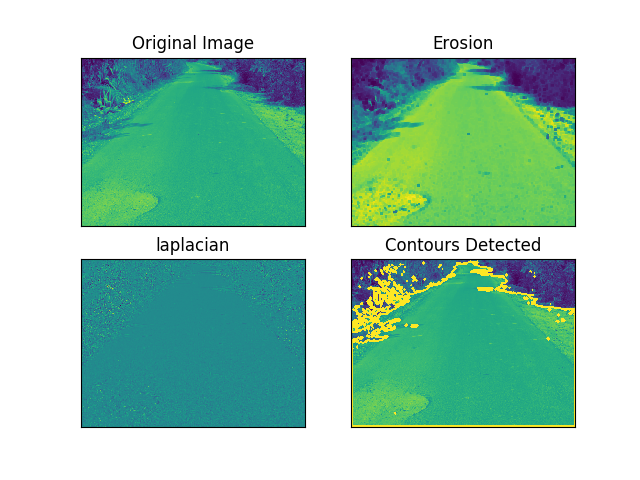
\includegraphics[width = 5in]{images/morph_transform_7.png}
        \caption{Output of Contour Detection using Morphological Transformation}
    \end{figure}
    \pagebreak
    
\end{itemize}

\vspace*{.5cm}



\newpage


In order to get dataset that is rooted in the real world, we went out and recorded 360p video of the roads in and around Electronic City phase 2. We managed to get about 20 minutes of footage of varying terrains with diverse features that are commonly encountered on Indian roads. The footage was preprocessed to reduce jitter induced in the video due to it being recorded by the pillion rider of a moving motorcycle. 

\vspace*{.25cm}

Collected data: \url{ https://youtu.be/hmeBmdZzlLU }

\vspace*{.25cm}

We expected the detection of potholes to be simplified if a localized area in the image can be found where the chance of occurrence of the pothole is relatively high. In essence, we decided to extract the road from the surrounding environment.

In order to remove the external environment and extract the road from the given frame, we tried a variety of techniques. 

\begin{itemize}

\item Choose a channel \\
    We had to come up with an input representation where the difference between the road and the surrounding was accentuated. We tried Grayscale images but the contrast wasn't enough to facilitate extraction. Much better results were found by converting the frame to HSV colorspace. We tried each channel in isolation and got satisfactory results with the S and V channels. 

 \begin{figure}[!ht]
\begin{center}

\begin{tabular}{ccc}
\centering
%\subfloat[Hue channel]{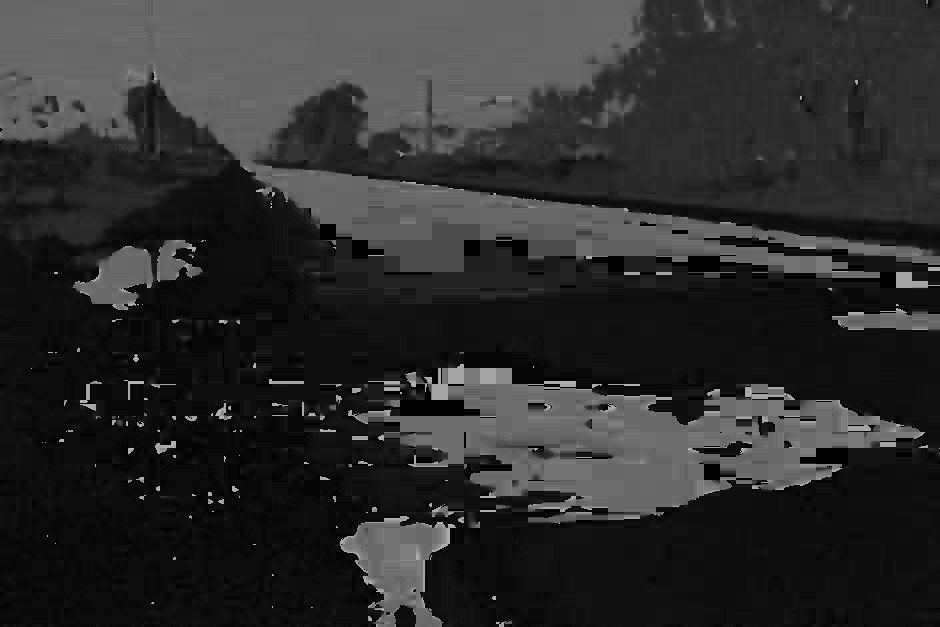
\includegraphics[width = 2in]{Hue.jpg}} &
%\subfloat[Saturation channel]{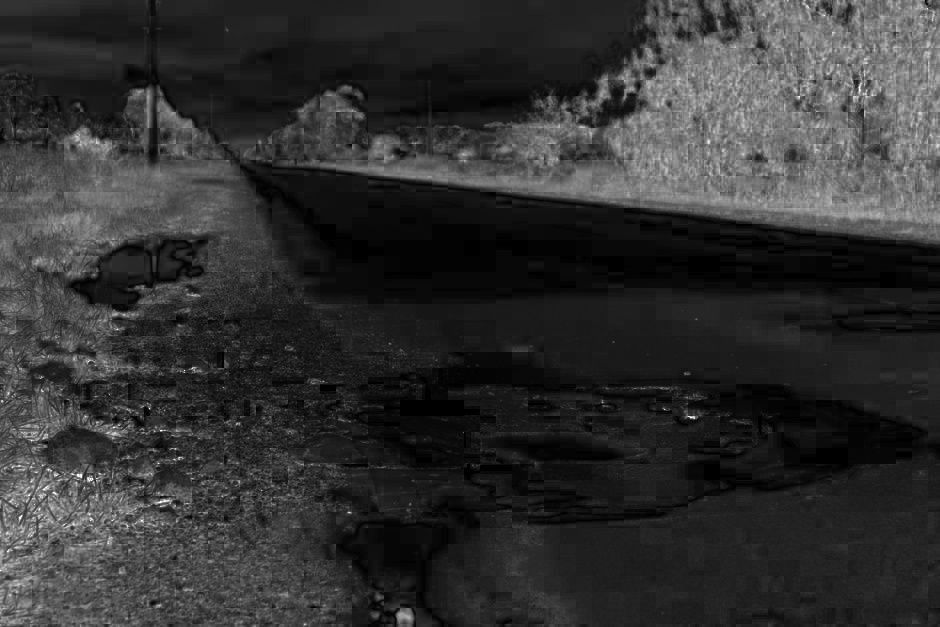
\includegraphics[width = 2in]{Saturation.jpg}} &
%\subfloat[Variance channel]{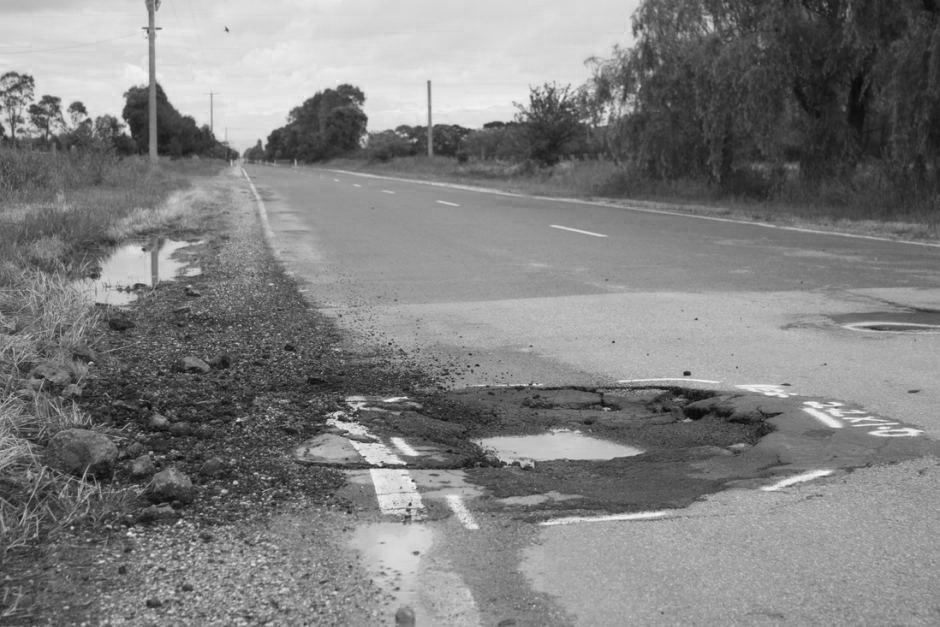
\includegraphics[width = 2in]{Variance.jpg}} 
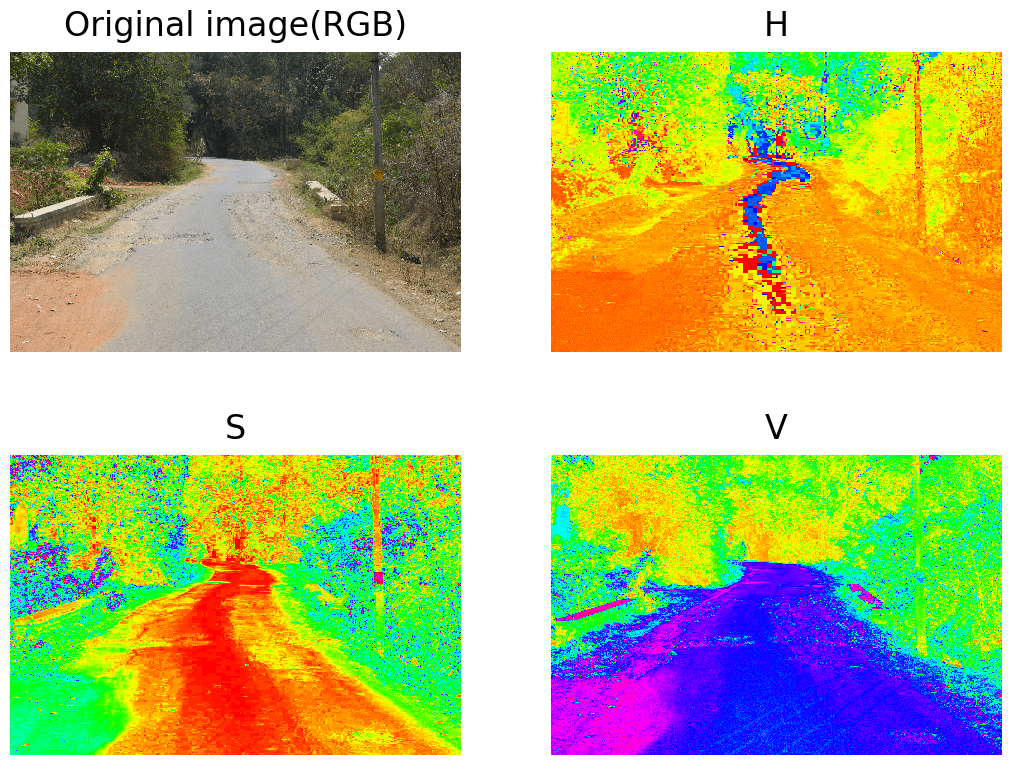
\includegraphics[width = 6in]{images/rgb_hsv_highdpi.png}
\end{tabular}
\caption{HSV channels for classic image}

\end{center}
\end{figure}

%\begin{figure}[ht!]
%\centering
%\begin{tabular}{ccc}
%\subfloat[Hue channel]{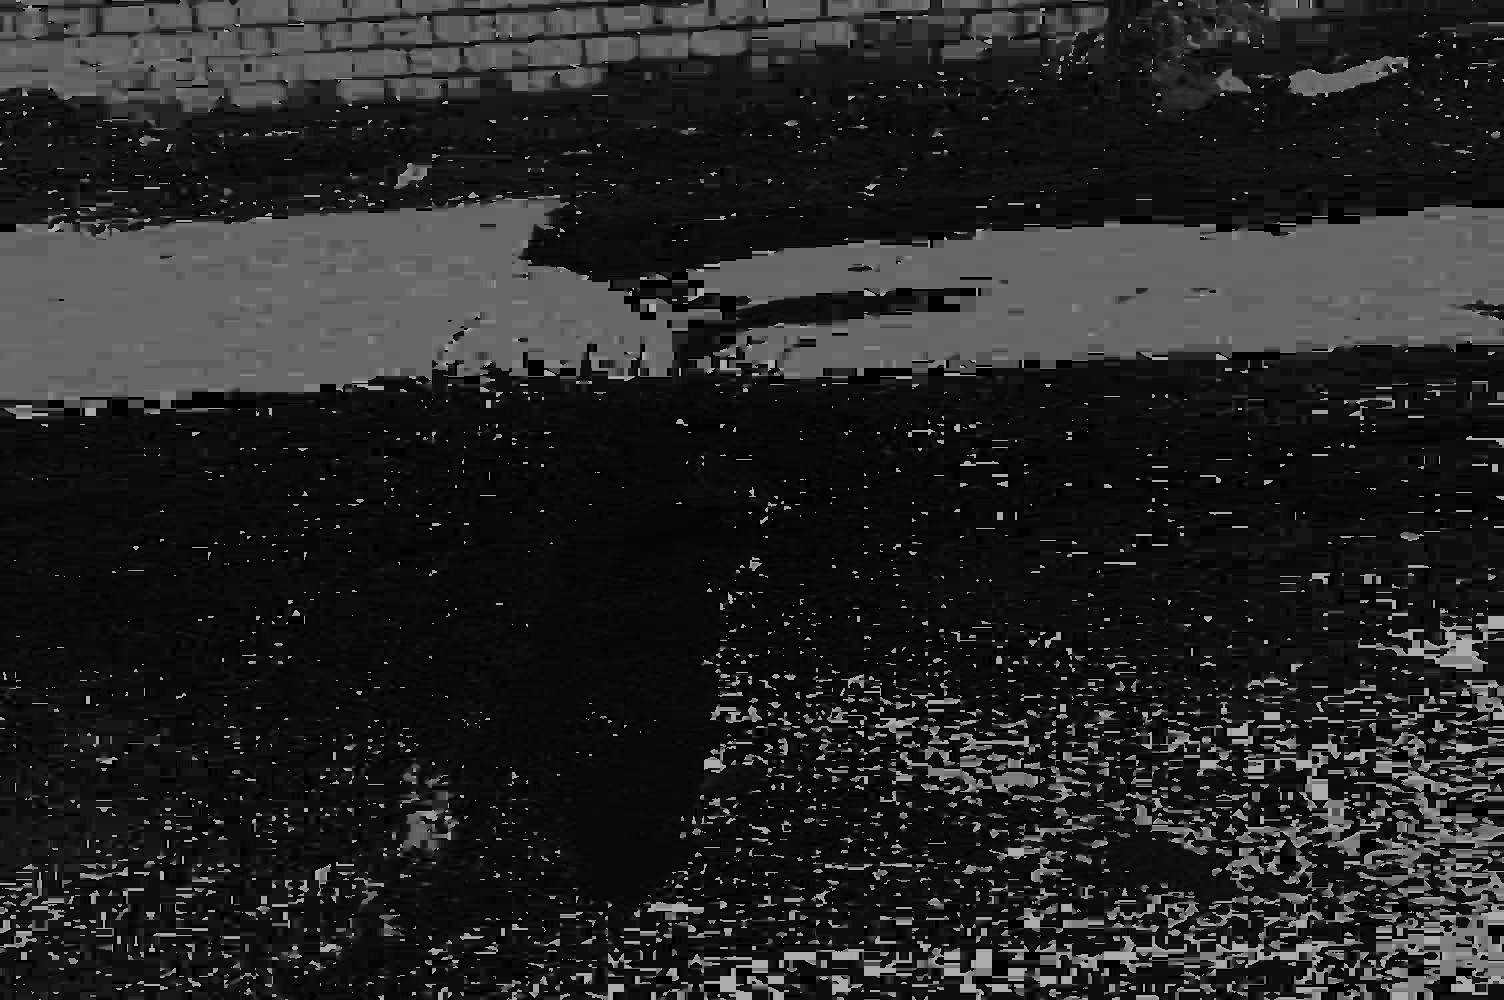
\includegraphics[width = 2in]{Hue_cam.jpg}} &
%\subfloat[Saturation channel]{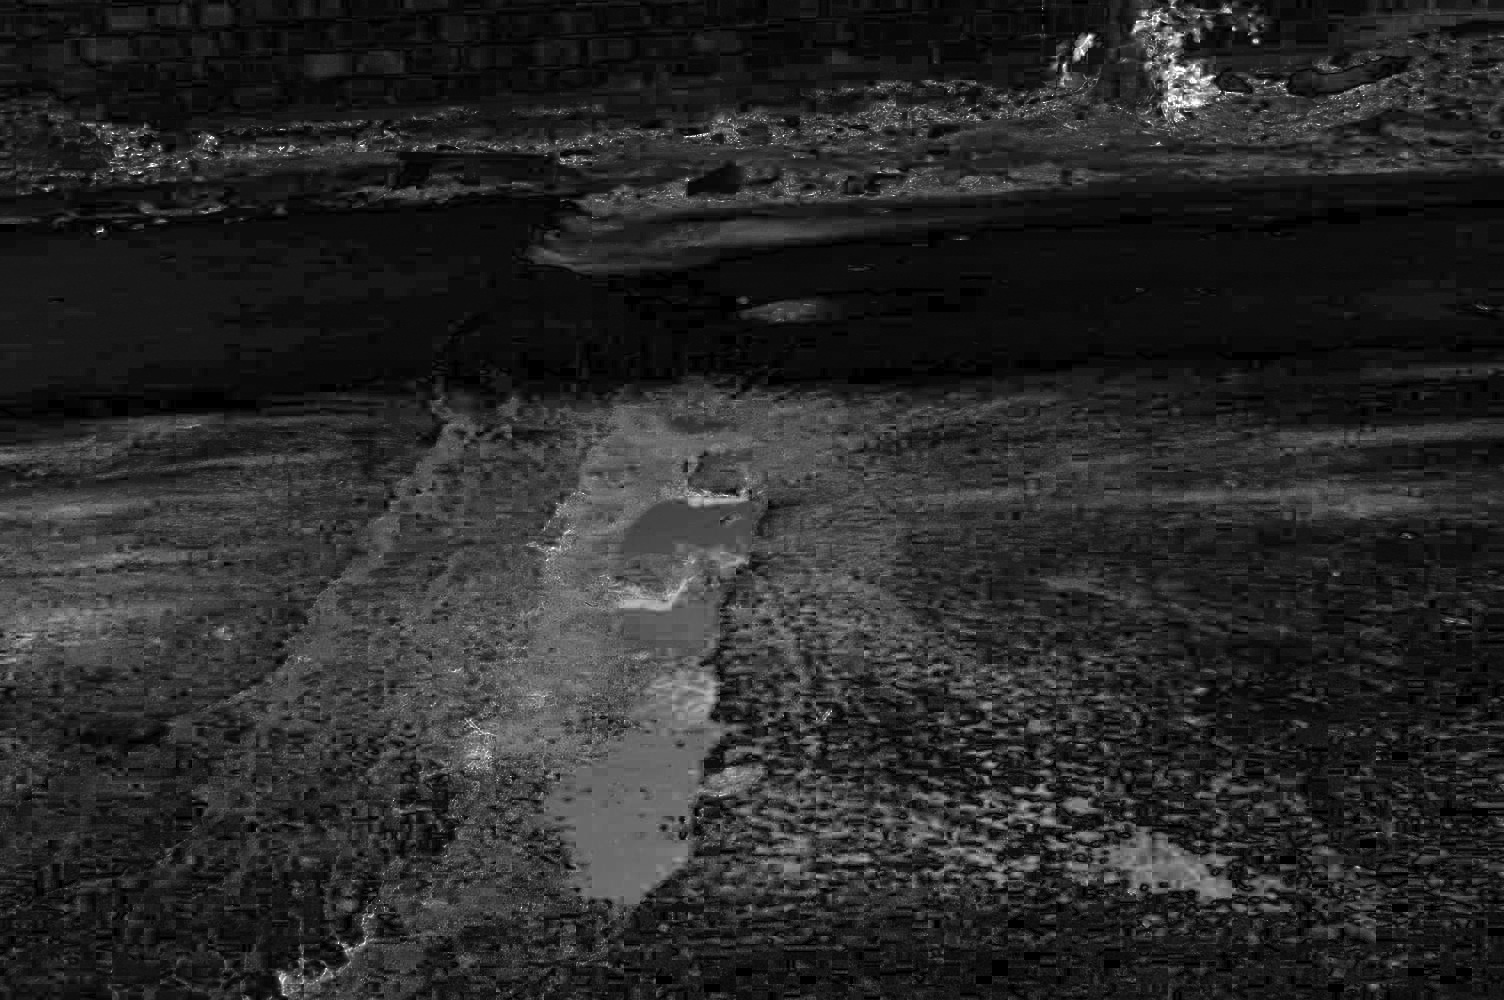
\includegraphics[width = 2in]{Saturation_cam.jpg}} &
%\subfloat[Variance channel]{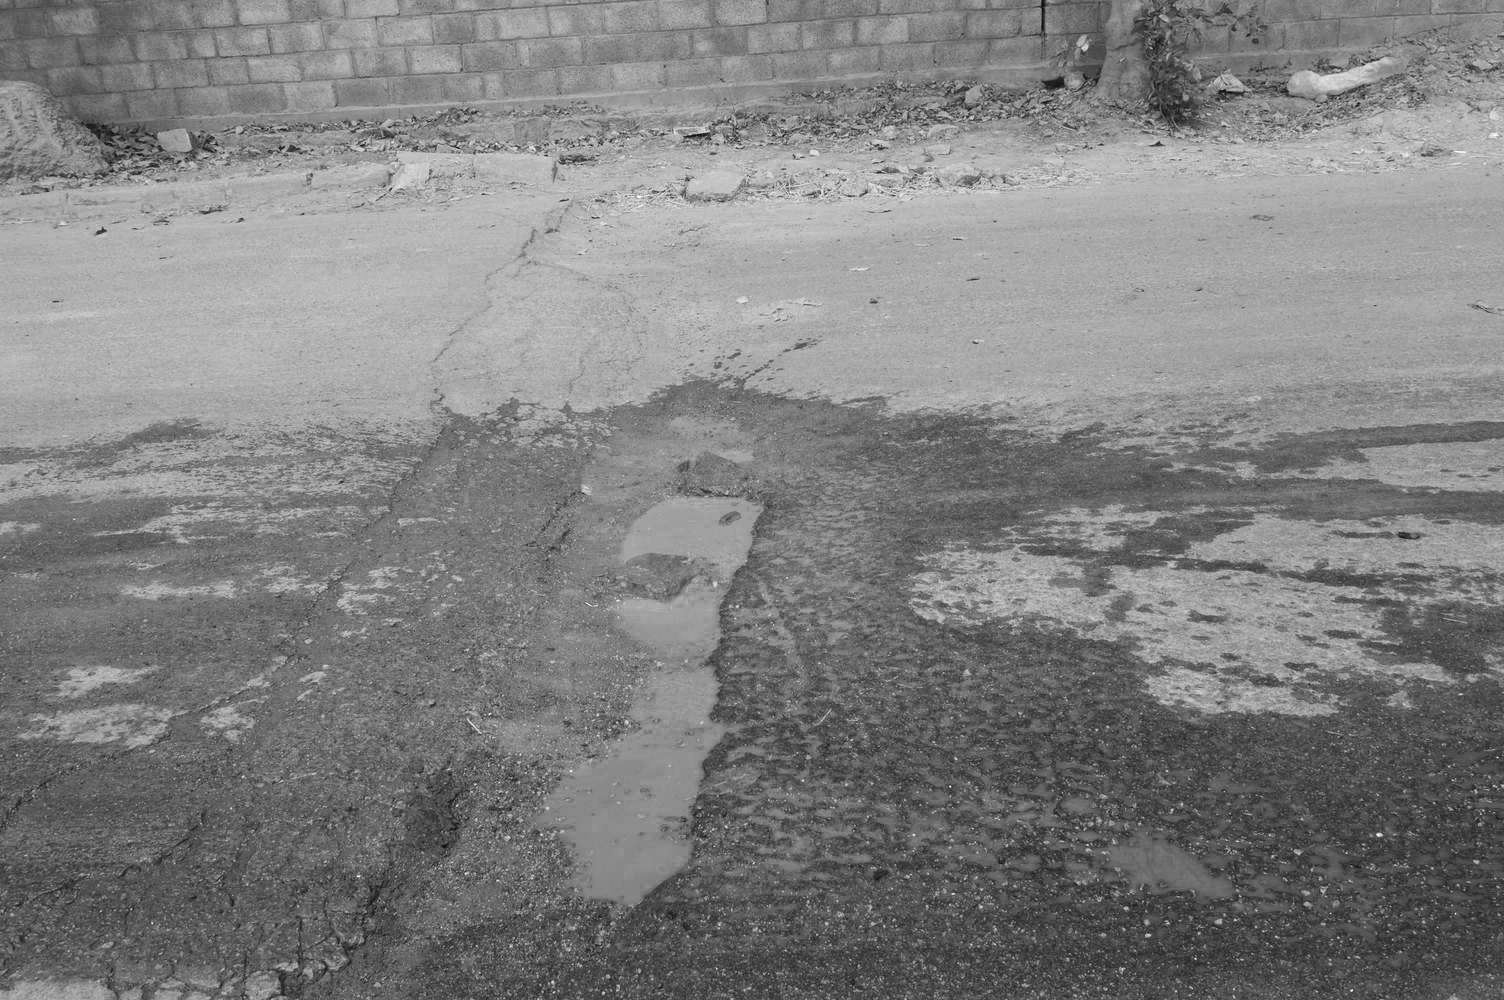
\includegraphics[width = 2in]{Variance_cam.jpg}}
%\end{tabular}
%\caption{HSV channels for collected dataset}
%\end{figure}
%     

\newpage
\item Remove Noise \\
    Now that we had a channel to work on, wee had to reduce the amount of noise in the frame. Between Gaussian Blur and Median Blur, we got better results with Median Blur with a relatively large kernel size to reduce the noise inherent in the picture. 

\item Threshold to get a suitable mask \\
    Now that we had a denoised version of the channel with maximum variance between the road and surrounding, we applied Otzu's thresholding to extract the part of the image containing the road. We got a relatively good output but there was still noise in the threshold mask.

\begin{figure}[!ht]
\begin{center}

\begin{tabular}{ccc}
\centering
%\subfloat[Hue channel]{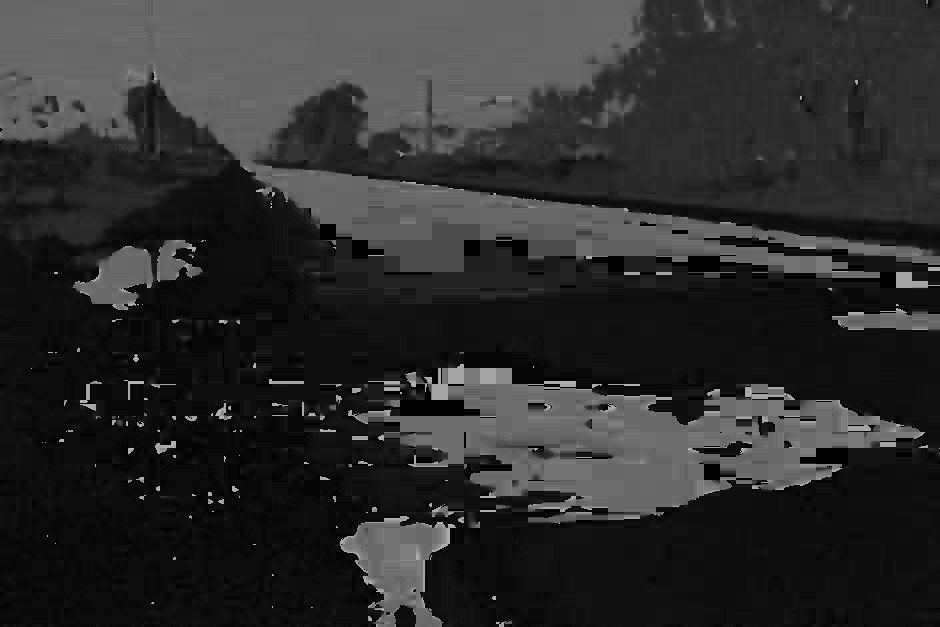
\includegraphics[width = 2in]{Hue.jpg}} &
%\subfloat[Saturation channel]{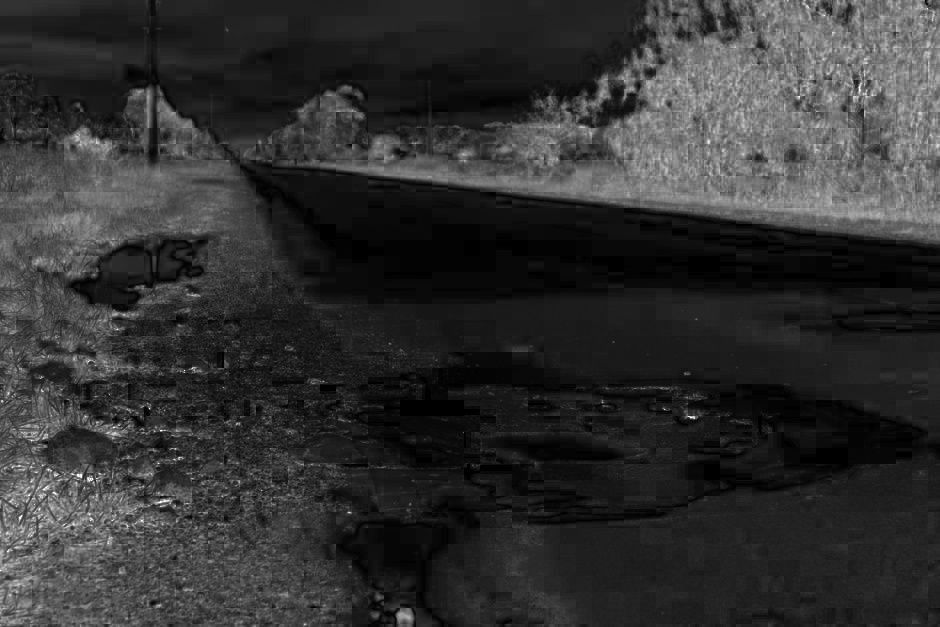
\includegraphics[width = 2in]{Saturation.jpg}} &
%\subfloat[Variance channel]{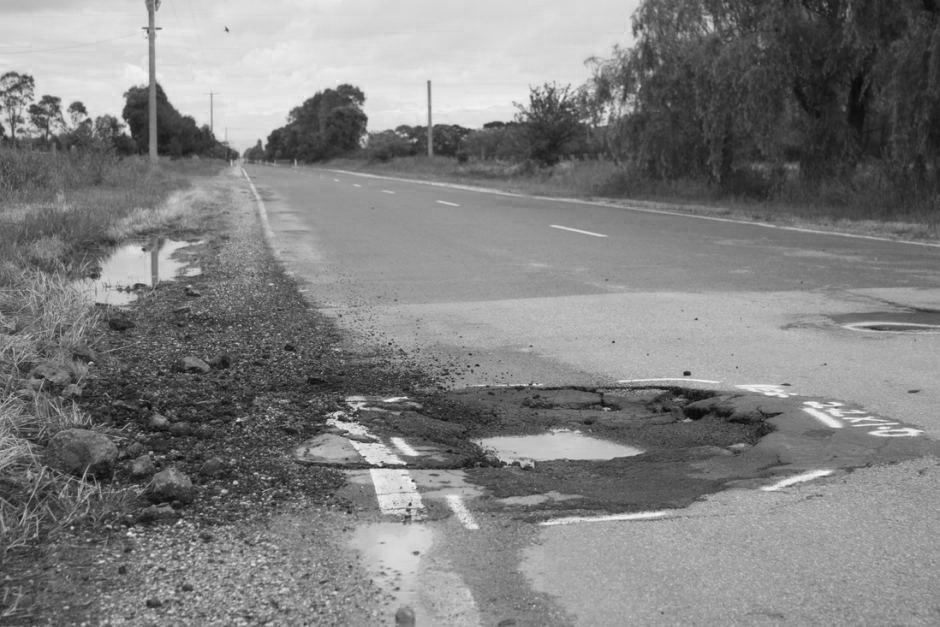
\includegraphics[width = 2in]{Variance.jpg}} 
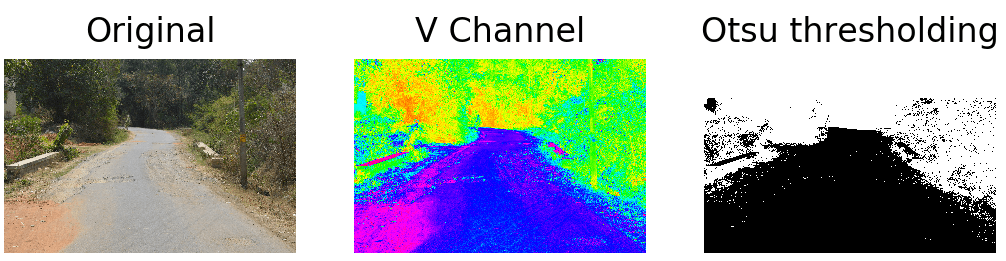
\includegraphics[width = 5.5in]{images/otzu_highdpi.png}
\end{tabular}
\caption{Thresholding to create a mask}

\end{center}
\end{figure}
    
\newpage
    
\item Clean up the mask \\
    Morphological transformations are some simple operations based on the image shape. It is normally performed on binary images. It needs two inputs, one is the original image, second one is called structuring element or kernel which decides the nature of operation. Two basic morphological operators are Erosion and Dilation. 
    ** Erosion: The basic idea of erosion is to erode away the boundaries of foreground object.  It is useful for removing small white noises, detach two connected objects etc.
    ** Dilation: It is just opposite of erosion. It increases the white region in the image or size of foreground object increases. Normally, in cases like noise removal, erosion is followed by dilation. Because, erosion removes white noises, but it also shrinks our object. So, we dilate it. Since noise is gone, they won't come back, but our object area increases. It is also useful in joining broken parts of an object. 
    
    There were still stray islands in the mask, i.e small localized black(white) regions within the white(black) areas. In order to even these out, we used the following two morphological transformation methods in succession -
    ** Closing : It is dilation followed by erosion. It is useful in closing small holes inside the foreground objects, or small black points on the object.
    ** Opening : It is erosion followed by dilation. It is useful in removing noise from the black areas.
    We used a relatively large kernel for both the operations to get a fairly clean mask.
 

\begin{figure}[!ht]
\begin{center}

\begin{tabular}{ccc}
\centering
%\subfloat[Hue channel]{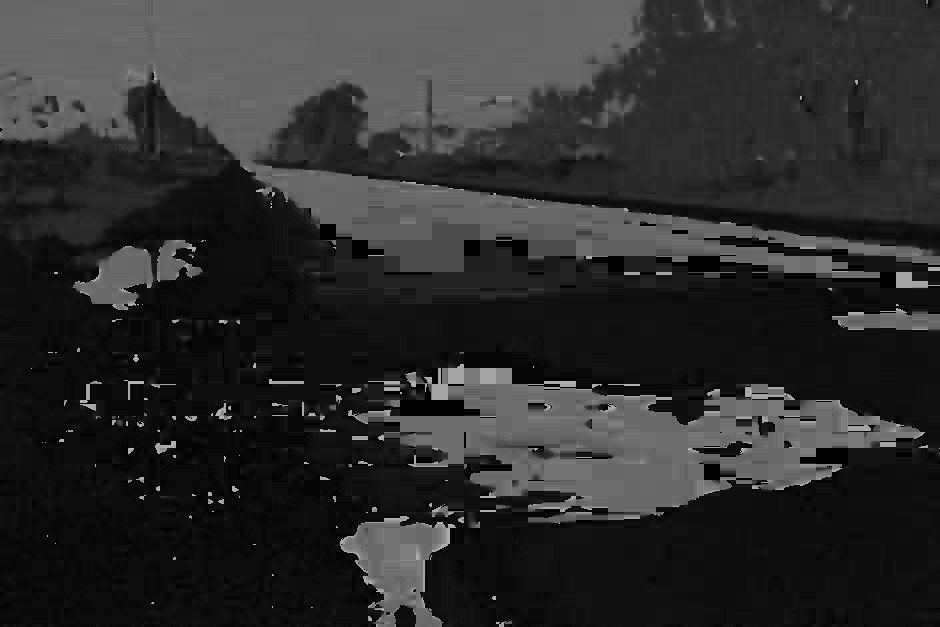
\includegraphics[width = 2in]{Hue.jpg}} &
%\subfloat[Saturation channel]{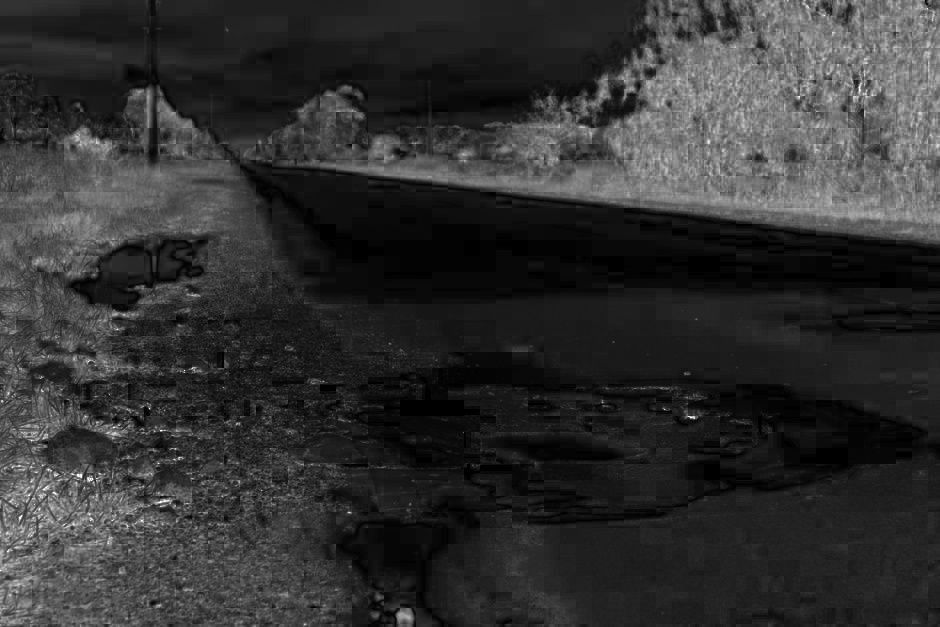
\includegraphics[width = 2in]{Saturation.jpg}} &
%\subfloat[Variance channel]{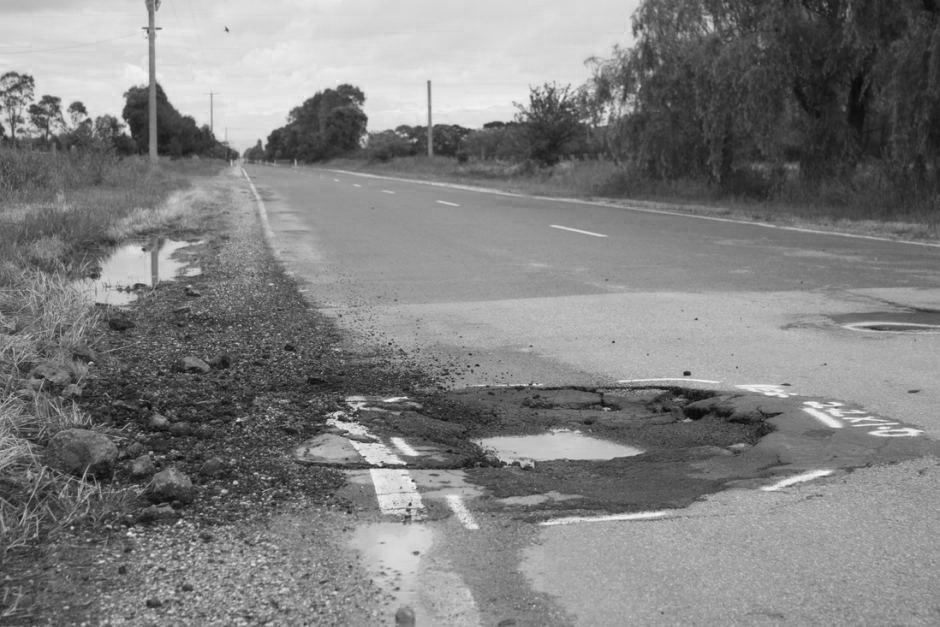
\includegraphics[width = 2in]{Variance.jpg}} 
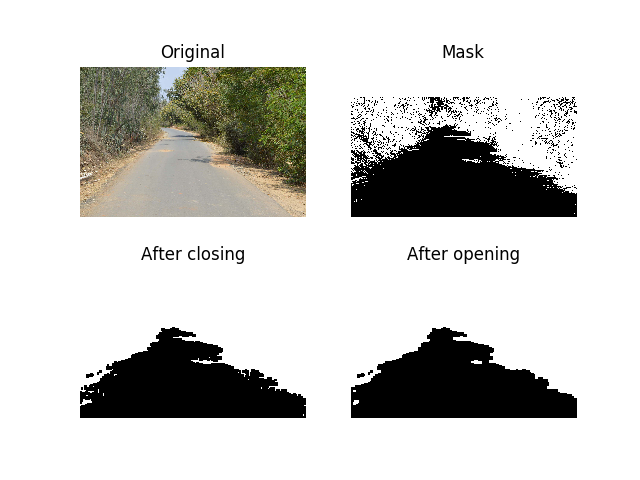
\includegraphics[width = 5in]{images/closing_opening.png}
\end{tabular}
\caption{Opening and Closing to clean up the mask}

\end{center}
\end{figure} 
\newpage

\item Application of mask \\
    The obtained mask was applied on the original image and the road was extracted out. 

\begin{figure}[!ht]
\begin{center}

\begin{tabular}{ccc}
\centering
%\subfloat[Hue channel]{\includegraphics[width = 2in]{Hue.jpg}} &
%\subfloat[Saturation channel]{\includegraphics[width = 2in]{Saturation.jpg}} &
%\subfloat[Variance channel]{\includegraphics[width = 2in]{Variance.jpg}} 
\includegraphics[width = 5in]{images/output.png}
\end{tabular}
\caption{Application of mask}

\end{center}
\end{figure} 

    Mask applied on collected dataset: \url{https://youtu.be/937GaZlRy2Y}.

    
\item Classic methods for edge detection
 
 We initially used some classic methods like k-means and meanshift for edge detection. While it worked good with the Google images, because of the zoomed and focused nature of potholes in the picture, there were challenges faced in clustering in our dataset because of real world problems,  like - sunlight, potholes filled with mud, making it hard to discern them from the roads. We concluded, therefore that dry and wet potholes cannot be preprocessed in a similar way, 
 
% \begin{figure}[ht!]
%\centering
%\begin{tabular}{ccc}
%\subfloat[Hue channel]{\includegraphics[width = 2in]{Hue_cam.jpg}} &
%\subfloat[Saturation channel]{\includegraphics[width = 2in]{Saturation_cam.jpg}} &
%\subfloat[Variance channel]{\includegraphics[width = 2in]{Variance_cam.jpg}}
%\end{tabular}
%\caption{HSV channels for collected dataset}
%\end{figure}
\newpage     
 
 \begin{figure}[ht!]
\centering
\begin{tabular}{ccc}
\subfloat[Original Google image]{\includegraphics[width = 2in]{road_10.jpg}} &
\subfloat[Clustered image]{\includegraphics[width = 2in]{Result_for_kmeans10.jpg}} 
\end{tabular}
\caption{K-means on classic Google images}
\end{figure}

 \begin{figure}[ht!]
\centering
\begin{tabular}{ccc}
\subfloat[Original Camera image]{\includegraphics[width = 2in]{road_cam_33.jpg}} &
\subfloat[Clustered image]{\includegraphics[width = 2in]{Result_for_camkmeans.jpg}} 
\end{tabular}
\caption{K-means on the dataset}
\end{figure}
    
\end{itemize}

\section{Future Work}
Future enhancements of this work is explained briefly in the following paragraph.


\subsection{Supervised Learning}
We will be generating manually labelled data from the images collected. Using the labelled image data we apply classical supervised learning techniques to find out the presence of potholes in the image. We will be extracting each frame separately from the video and segregate the frames that has potholes. SURF or SIFT detectors are used to extract features from the images which is used for learning. 

\subsection{Classification}
After the features are extracted we using various machine learning techniques to classify whether or not the given frame from a video contains potholes. We use methods like Naive Bayes, KNearest Neighbour, SVM and the like to train the model and predict the existence of the potholes.


\subsection{Comparative analysis}
A study is then done based on the result obtained from the classical machine learning methods to find out which method works best in a given scenario.

\begin{thebibliography}{9}
\bibitem{paperone} 
S Nienaber*, M Booysen* AND R Kroon**.
\textit{Detecting potholes using simple image processing techniques and Real-world Footage, 2015}. 
*Department of E\&E Engineering, Stellenbosch University.
**Computer Science Division, Stellenbosch University
\url{http://scholar.sun.ac.za/handle/10019.1/97191}
 
\bibitem{papertwo} 
Ajit Danti, Jyoti Y. Kulkarni, and P. S. Hiremath, Member, IACSIT
\textit{An Image Processing Approach to Detect Lanes, Pot Holes and Recognize Road Signs in Indian Roads, December 2012}
\url{http://www.ijmo.org/papers/204-S3015.pdf}
\end{thebibliography}

\end{document}

